\documentclass[IN,11pt,twoside,openright,master,english]{tumthesis}

% Include common packages
\usepackage{packages}

% IEEE tools for tweaking bib style
\usepackage{IEEEtrantools}

\newcommand\toc{\relax}

\usepackage[backend=bibtex]{biblatex}
\usepackage{booktabs}
\usepackage{tabularx}
\usepackage{longtable}
\usepackage{tabu}
\usepackage{ltxtable}
\usepackage{url}
\usepackage[style=base]{caption}
\captionsetup{%
	font={rm,footnotesize},
	labelfont={sc},
}
\captionsetup[subfloat]{%
	font={rm,footnotesize},
	labelfont={rm},
}
\usepackage{subfig}
\usepackage{nicefrac}
\usepackage{longtable}
\usepackage[hang]{footmisc}
\usepackage[version=2]{acro}
\usepackage{blindtext}

\setlength\footnotemargin{5pt}

% Theorem environments
\newtheorem{definition}{Definition}
\newtheorem{theorem}{Theorem}
\newtheorem{example}{Example}
\newtheorem{lemma}{Lemma}


% hyphenation
\hyphenation{op-ti-cal net-work net-works semi-con-duc-tor tech-nique tech-niques}


\usepackage{mdframed}
\newlength{\charwidth}
\setlength{\charwidth}{\widthof{\scriptsize\texttt{x}}}

\makeatletter
\newenvironment{moeplstborder}[2][]{%
\ifx#1\@empty\@empty%
	\edef\@margin{-1.5\baselineskip}%
\else%
	\edef\@margin{#1}%
\fi%
\vspace{-\baselineskip}
\begin{center}
\begin{minipage}{#2}
\begin{mdframed}[%
	topline=false,leftline=false,bottomline=false,rightline=true,
	linecolor=TUMRed!20,linewidth=\charwidth,
	innertopmargin=\@margin,innerbottommargin=-0.5\baselineskip,
	innerleftmargin=0pt,innerrightmargin=-\charwidth,
	userdefinedwidth=#2,
]%
}%
{%
\end{mdframed}%
\end{minipage}
\end{center}
}%
\makeatother

% Needed for Bachelor's theses, Master's theses and IDP
\titleenglish{Investigating effects of hardware isolation in high-speed network environments}
\titlegerman{Auswirkungen von Hardware-Isolation in Hochgeschwindigkeits-Netzwerkumgebungen}
\author{Simon~Ellmann}
\supervisor{\NEThead}
\advisor{Prof.~Dr.-Ing.~Wolfgang~Utschick}
%\assistants{Dipl.-Ing.~Stephan~M.~G\"unther\tlc{}~M.\,Sc.,%
%Maurice~Leclaire\tlc{}~M.\,Sc.}
\assistants{Paul~Emmerich\tlc{}~M.\,Sc.,%
Florian~Wiedner\tlc{}~M.\,Sc.,%
Benedikt~J\"ager\tlc{}~M.\,Sc.}

% in case of bachelor's/master's thesis use your own field of study
%\courseofstudy{Informatik}
\courseofstudy{Informatics}
%\courseofstudy{Informatik: Games Engineering}
%\courseofstudy{Informatics: Games Engineering}

% in case of idp use electrical engineering as your field of study
%\courseofstudy{Elektrotechnik}
%\courseofstudy{Electrical Engineering}

\date{April 15, 2021}
\location{Garching}

\setcounter{tocdepth}{2}

\DeclareAcroListStyle{longtabu}{table}{%
	table = longtabu,
	table-spec = @{}>{}lX@{}
}{%

\acsetup{%
	list-style=longtabu,
	extra-style=plain,	% remove dot after long in list
	only-used=false,
}

\tabulinesep=1ex

\DeclareAcronym{io}{
    short               = {\sc{I/O}},
    long                = {input/output},
    list                = {\Acl{io}.},
    extra               = {%
        Flow of information between an information processing system and a human
        or another information processing system.
    }
}
\DeclareAcronym{cpu}{
    short               = {\sc{CPU}},
    short-plural-form   = {\sc*{CPU}s},
    long                = {central processing unit},
    long-plural-form    = {central processing units},
    list                = {\Acl{cpu}.},
    extra               = {%
        Electronic circuitry that executes arithmetic, logic, control and
        \acs{io} instructions specified by computer programs.
    }
}
\DeclareAcronym{dma}{
    short               = {\sc{DMA}},
    long                = {direct memory access},
    list                = {\Acl{dma}.},
    extra               = {%
        Feature of computer systems that allows hardware to access main memory
        independent of the \acs{cpu}.
    }
}
\DeclareAcronym{sriov}{
    short               = {\sc{SR-IOV}},
    long                = {single root input/output virtualization},
    list                = {\Acl{sriov}.},
    extra               = {%
        Feature of computer systems that allows a single \ac{pcie} device to be
        shared with multiple virtual environments.
    }
}
\DeclareAcronym{mmu}{
    short               = {\sc{MMU}},
    short-plural-form   = {\sc*{MMU}s},
    long                = {memory management unit},
    long-plural-form    = {memory management units},
    list                = {\Acl{mmu}.},
    extra               = {%
        Computer hardware component that primarily translates virtual to
        physical memory addresses. Often part of the \ac{cpu}.
    }
}
\DeclareAcronym{iommu}{
    short               = {\sc{IOMMU}},
    short-plural-form   = {\sc*{IOMMU}s},
    long                = {input-output memory management unit},
    long-plural-form    = {input-output memory management units},
    list                = {\Acl{iommu}.},
    extra               = {%
        A \ac{mmu} for \ac{io} devices.
    }
}
\DeclareAcronym{tlb}{
    short               = {\sc{TLB}},
    short-plural-form   = {\sc*{TLB}s},
    long                = {translation lookaside buffer},
    long-plural-form    = {translation lookaside buffers},
    list                = {\Acl{tlb}.},
    extra               = {%
        Memory cache of a \ac{mmu} that stores recent address translations to
        improve performance.
    }
}
\DeclareAcronym{iotlb}{
    short               = {\sc{IOTLB}},
    short-plural-form   = {\sc*{IOTLB}s},
    long                = {I/O translation lookaside buffer},
    long-plural-form    = {I/O translation lookaside buffers},
    list                = {\Acl{iotlb}.},
    extra               = {%
        \ac{tlb} of an \ac{iommu}.
    }
}
\DeclareAcronym{nic}{
    short               = {\sc{NIC}},
    short-plural-form   = {\sc*{NIC}s},
    long                = {network interface controller},
    long-plural-form    = {network interface controllers},
    list                = {\Acl{nic}.},
    extra               = {%
        Computer hardware component that receives and transmits data via a
        computer network.
    }
}
\DeclareAcronym{os}{
    short               = {\sc{OS}},
    short-plural-form   = {\sc*{OS}es},
    long                = {operating system},
    long-plural-form    = {operating systems},
    list                = {\Acl{os}.},
    extra               = {%
        Low-level software that manages a computer's hardware and software and
        provides services for computer programs.
    }
}
\DeclareAcronym{pcie}{
    short               = {\sc{PCIe}},
    long                = {Peripheral Component Interconnect Express},
    list                = {\Acl{pcie}.},
    extra               = {%
        High-speed serial bus standard designed to replace PCI.
    }
}
\DeclareAcronym{bios}{
    short               = {\sc{BIOS}},
    short-plural-form   = {\sc*{BIOS}es},
    long                = {Basic Input/Output System},
    long-plural-form    = {Basic Input/Output Systems},
    list                = {\Acl{bios}.},
    extra               = {%
        Firmware that initializes a computer's hardware on boot before the
        \ac{os} is loaded.
    }
}
\DeclareAcronym{uefi}{
    short               = {\sc{UEFI}},
    long                = {Unified Extensible Firmware Interface},
    list                = {\Acl{uefi}.},
    extra               = {%
        Standardized successor of the \acp{bios} found in IBM PC-compatible
        computers.
    }
}
\DeclareAcronym{vfio}{
    short               = {\sc{VFIO}},
    long                = {Virtual Function I/O},
    list                = {\Acl{vfio}.},
    extra               = {%
        Linux driver framework that utilizes \acp{iommu} and allows direct
        device access from userspace in a safe manner.
    }
}
\DeclareAcronym{iova}{
    short               = {\sc{IOVA}},
    short-plural-form   = {\sc*{IOVA}s},
    long                = {I/O virtual address},
    long-plural-form    = {I/O virtual addresses},
    list                = {\Acl{iova}.},
    extra               = {%
        Address used by \ac{io} devices for \ac{dma} access. \acp{iommu}
        translate IOVAs to physical adresses.
    }
}
\DeclareAcronym{acpi}{
    short               = {\sc{ACPI}},
    long                = {Advanced Configuration and Power Interface},
    list                = {\Acl{acpi}.},
    extra               = {%
        Open standard for discovery and configuration of computer hardware
        components by \acp{os}.
    }
}
\DeclareAcronym{dmar}{
    short               = {\sc{DMAR}},
    long                = {DMA remapping},
    list                = {\Acl{dmar}.},
    extra               = {%
        Component of \acp{iommu} responsible for address translation. Often
        used synonymously with \ac{iommu}.
    }
}
\DeclareAcronym{vf}{
    short               = {\sc{VF}},
    short-plural-form   = {\sc*{VF}s},
    long                = {virtual function},
    long-plural-form    = {virtual functions},
    list                = {\Acl{vf}.},
    extra               = {%
        Lightweight \ac{pcie} function of \ac{sriov}-capable devices that can
        be passed-through to a virtual environment.
    }
}
\DeclareAcronym{pf}{
    short               = {\sc{PF}},
    short-plural-form   = {\sc*{PF}s},
    long                = {physical function},
    long-plural-form    = {physical functions},
    list                = {\Acl{pf}.},
    extra               = {%
        Fully featured \ac{pcie} function that supports \ac{sriov} and creates
        and manages one or multiple \acp{vf} when required.
    }
}
\DeclareAcronym{bdf}{
    short               = {\sc{BDF}},
    long                = {bus/device/function number},
    list                = {\Acl{bdf}.},
    extra               = {%
        Identifier triple of \ac{pcie} devices.
    }
}
\DeclareAcronym{mac}{
	short				= {\sc{MAC}},
	long				= {medium access control},
	list				= {\Acl{mac}.},
    extra               = {%
        Sublayer of the data link layer responsible for flow control and
        multiplexing of the transmission medium.
    }
}


\addbibresource{bib/IEEEfull.bib}
\addbibresource{bib/litnew.bib}


%\renewcommand{\andothersdelim}{}
%bib.sty does not work older bibtex versions (works on TexLive 2016 or newer)
%\usepackage{bib}

% Load late to avoid same identifier warning
\usepackage[colorlinks=false,pdfborder={0 0 0}]{hyperref}

\usepackage{bytefield}
\usepackage{listings-rust}
\usepackage{multirow}
\usepackage[nameinlink]{cleveref}

\renewcommand{\lstlistlistingname}{List of Listings}

\begin{document}%

% Makes sure that same author names are not replaced by dahes
\bstctlcite{IEEEexample:BSTcontrol}

\pagenumbering{gobble}
\maketitle%
\cleardoublepage


\begin{abstract}
	\small

Hardware isolation plays an important role in today's computer systems.
Internet companies and telecommunication providers rely on it for their heavily
virtualized infrastructures with \acl{sdn}, \acl{nfv}, containers and virtual
machines, and consumer hardware uses it to protect itself against malicious or
faulty external peripherals.

One common way to isolate hardware is the use of \acp{iommu}, multipurpose
devices to virtualize \acs{io} memory that can be found in all kinds of devices
nowadays, from high-end servers to mobile devices like Apple's iPhones, and are
inevitable for fast \ac{io} on platforms like Amazon's Elastic Cloud Computing.
Due to their widespread use, questions arise whether \acp{iommu} impact
performance and safety/security of the systems they are used in.

We address these questions in the area of high-speed network environments. For
our analyses, we use \texttt{ixy.rs}, a state-of-the-art user space network
driver for Intel's 82599 network cards written in Rust. We show that \acp{iommu}
have a minor impact on performance in most cases. In some cases, however,
\acp{iommu} lead to a loss of packet throughput of more than 50\%. While our
suspicion of a side-channel vulnerability in the \aclp{tlb} of \acp{iommu} is
not confirmed, we note that \ac{iommu} protection against malicious peripherals
is weak.

Our contributions are a new driver to \texttt{ixy.rs} for \aclp{vf}, support for
legacy Intel \acp{iommu} with limited second-level address translation
capabilities, and a tool to perform accurate timing measurements on network card
\acs{dma} operations. Besides, we have fixed an error in DPDK's ixgbevf driver.


\end{abstract}

\begin{otherlanguage}{ngerman}
	\begin{abstract}
		\small

Hardware-Isolation spielt in heutigen Computersystemen eine wichtige Rolle.
Internetfirmen und Telekommunikationsanbieter sind mit ihrer stark
virtualisierten Infrastruktur auf Hardware-Isolation angewiesen, und
Verbraucherprodukte nutzen sie, um sich vor böswilligen oder fehlerhaften
externen Geräten zu schützen.

Eine gängige Methode zur Isolierung von Hardware ist die Verwendung von IOMMUs,
Mehrzweckgeräten zur Virtualisierung von IO-Speicher, die heutzutage in allen
Arten von Geräten zu finden sind, von High-End-Servern bis hin zu mobilen
Geräten wie Apples iPhones, und die für schnelle IO-Operationen auf Plattformen
wie Amazons Elastic Cloud Computing unumgänglich sind. Aufgrund der weiten
Verbreitung von IOMMUs stellt sich die Frage, inwiefern sie die Leistung und die
Sicherheit der Systeme, in denen sie eingesetzt werden, beeinflussen.

Wir adressieren diese Frage im Bereich von
Hochgeschwindigkeits-Netzwerkumgebungen. Für unsere Analyse verwenden wir
\texttt{ixy.rs}, einen in Rust geschriebenen, modernen
User-Space-Netzwerktreiber für Intels 82599-Netzwerkkarten. Wir zeigen, dass
IOMMUs in den meisten Fällen einen geringen Einfluss auf die Performance haben.
In manchen Fällen jedoch führen IOMMUs zu einem Performanceverlust von mehr als
50\%. Während sich unser Verdacht auf eine Seitenkanal-Schwachstelle in den
Übersetzungspuffern von IOMMUs nicht bestätigt, stellen wir fest, dass der
Schutz von IOMMUs gegenüber bösartigen Geräten gering ist.

Mit dieser Arbeit tragen wir einen neuen Treiber zu \texttt{ixy.rs} für
virtuelle Funktionen, Unterstützung für ältere Intel-IOMMUs mit eingeschränkter
Second-Level-Adressübersetzung und ein Werkzeug zur Durchführung genauer
Zeit-Messungen auf Speicherzugriffe von Netzwerkkarten bei. Des Weiteren wurde
ein Fehler in DPDKs ixgbevf-Treiber behoben.


	\end{abstract}
\end{otherlanguage}

\begin{thanks}
        \small

First and foremost, I would like to thank my supervisor,
Prof.~Dr.-Ing.~Georg~Carle, for his enduring support and confidence in my
abilities, for the opportunity to conduct research at his chair, for our
discussions on my work, and for enabling me to participate in conferences and
workshops.

I would like to say a special thank you to Paul Emmerich for all the pleasurable
conversations, his moral support, and the invaluable feedback on my work. His
profound knowledge and enthusiasm for research made my time at the chair all the
more enjoyable.

I also wish to thank Florian Wiedner and Benedikt Jaeger for their guidance and
feedback, which contributed significantly to the success of this thesis.

Furthermore, I would like to thank Heiko Simoneit, Catharina Großmaß and Clemens
Horn for their friendship, unclouded optimism in all circumstances and our
leisure activities.

And last but not least, I would like to express my deep gratitude to my family
for their unconditional support throughout the last years.


\end{thanks}

\tableofcontents
\startcontent


\chapter{Introduction}
\label{chap:introduction}

TODO



\chapter{Background}
\label{chap:background}

\Ac{io} devices interact with the \acs{cpu} via interrupts, registers and shared
memory. We provide an overview of how these communication primitives work with
\acp{iommu} in context of network environments in the following sections,
focusing on \acs{pcie}, \acsp{nic}, \acsp{iommu} on Linux, and \acs{sriov}.


\section{Overview}
\label{sec:overview}

\begin{figure}[!b]
    \centering
    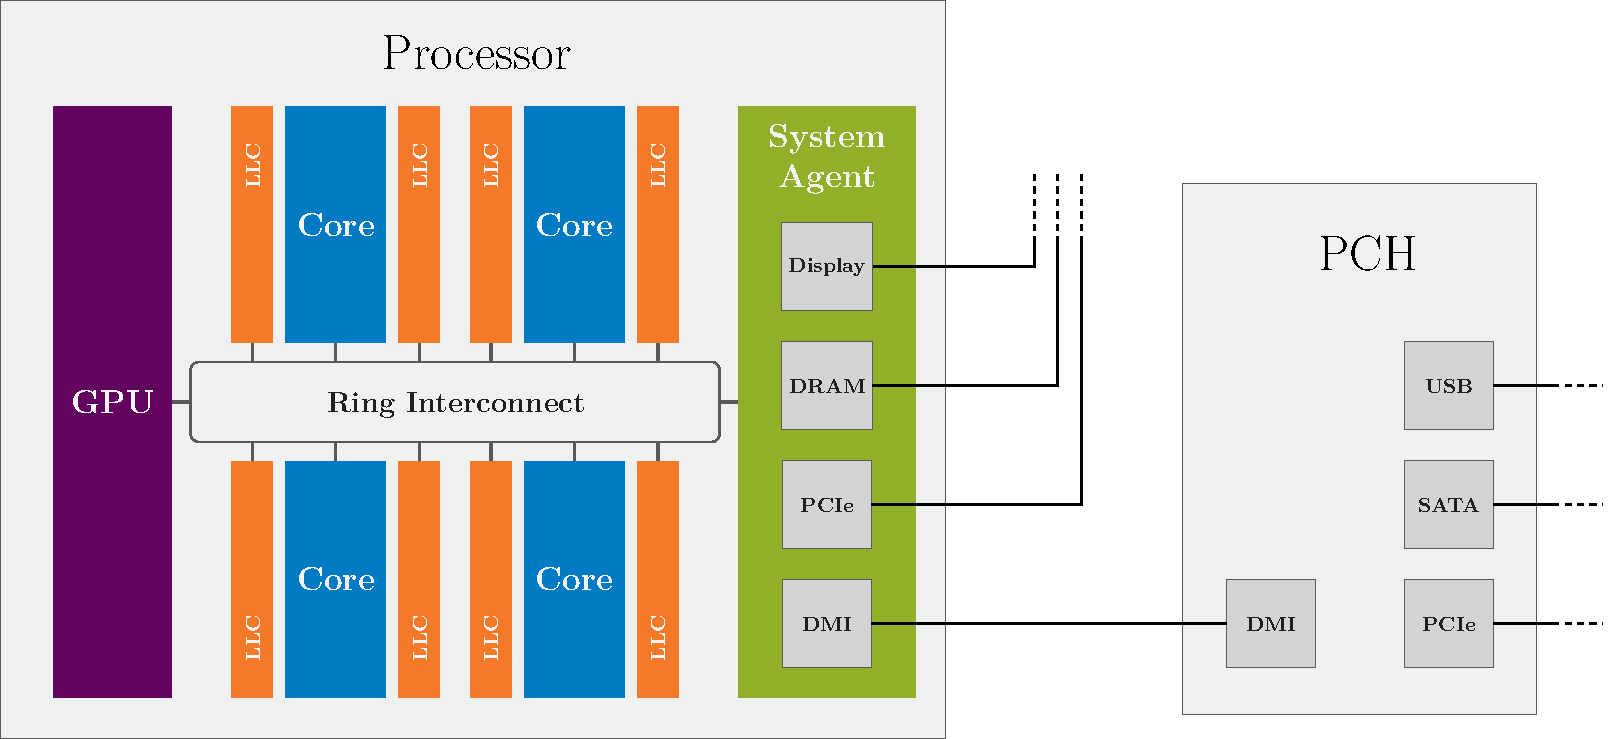
\includegraphics[width=0.8\textwidth]{figures/cpu-and-pch}
    \caption{Processor and Platform Controller Hub (PCH) on an Intel system.}
    \label{fig:pch}
\end{figure}

On modern systems, peripherals, processor and main memory are interconnected via
a wide set of connection standards and protocols. Devices are either directly
attached to the \ac{cpu} via \ac{pcie} or to an \acs{io} hub known as Platform
Controller Hub~(Intel) or chipset~(AMD). Direct connections are preferred for
\ac{io} devices with high performance requirements such as video cards or NVMe
controllers. On enterprise hardware, e.g., servers, most \ac{pcie} devices are
directly attached to the \ac{cpu}, whereas the \ac{io} hub is connected to
slower peripherals like on-board Gigabit network cards. On consumer hardware,
more devices are usually attached to the \ac{io} hub. The \ac{io} hub resides on
a separate chip and is connected to the \ac{cpu} via Direct Media Interface
(Intel) or Unified Media Interface (AMD). \Cref{fig:pch} illustrates the
relationship between \ac{cpu}, \ac{io} hub and peripherals. Conceptually, system
agent and Platform Controller Hub (PCH) depicted in \Cref{fig:pch} are
successors of northbridge and southbridge from previous chipsets. While memory
controller and other northbridge functions were incorporated into the \ac{cpu}
as so-called system agent, southbridge and remaining northbridge functions were
moved to the PCH.


\section{PCI Express}
\label{sec:pcie}

As de-facto standard, \acf{pcie} is used for communication with most
peripherals. \ac{pcie} is a high-speed serial bus that was designed to replace
PCI and PCI-X. Unlike the former, \ac{pcie} is based on a point-to-point
topology where all communication data is encapsulated in \ac{pcie} packets, and
supports hotplugging of devices. Conceptually, \ac{pcie} consists of various
communication layers and -- similar to TCP -- provides mechanisms like flow
control and acknowledgement messages to ensure reliable data transmission.

Physically, \ac{pcie} devices are connected via lanes which consist of two
differential pairs each, i.e., four wires per lane. The two pairs of \ac{pcie}
lanes are used unidirectionally as one transmit and one receive channel.
Together, they form a bidirectional link. For interrupts, no physical pin is
used. Instead, in-band messages signal interrupts to the interrupt controller
which in turn interrupts the \ac{cpu}. To increase throughput, devices may use
up to 32 lanes. With today's commonly used \ac{pcie} 4.0 (which was released in
2017), a serial data rate of \SI{16}{\Gbps} per lane or
\SI{1.97}{\giga\byte\per\second} (taking the 128b/130b line code into account)
can be achieved. Compared to \ac{pcie} 1.0 (released in 2003), throughput of the
lanes has increased by a factor of eight.

\begin{figure}
    \centering
    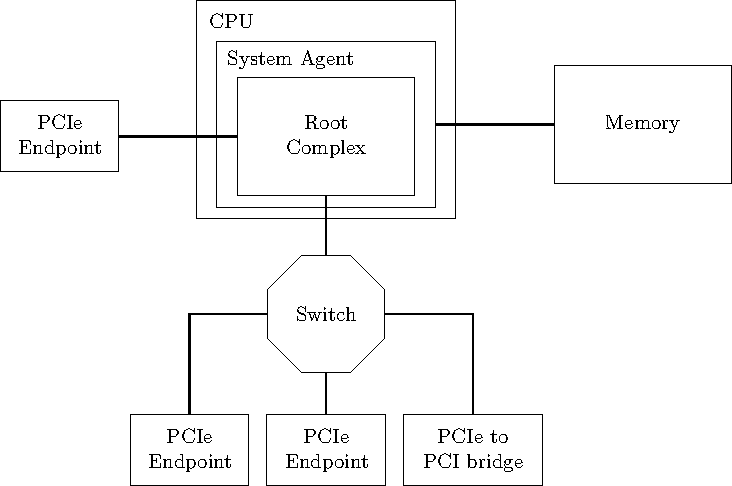
\includegraphics[width=0.6\textwidth]{figures/pcie-tree}
    \caption{Exemplary \acs{pcie} topology on an Intel system.}
    \label{fig:pcie-topology}
\end{figure}

Between \ac{pcie} devices and processor, switches may be used.
\Cref{fig:pcie-topology} depicts a typical \ac{pcie} tree. On the \ac{cpu} side,
connections end in the \ac{pcie} root complex which is part of the system agent
on Intel systems and the bridge between \ac{cpu}, main memory and devices. On
the device side, connections end at \ac{pcie} endpoints. \ac{pcie} devices may
initiate transfers to main memory through the \ac{pcie} root complex, acting as
\acs{dma} bus masters that access main memory independently of the \ac{cpu}.

\ac{pcie} uses three layers for communication: a physical layer, a data link
layer and a transaction layer. The physical layer of \ac{pcie} is responsible
for link initialization and point-to-point data transfer. The data link layer
ensures reliable transport of data between individual \ac{pcie} endpoints, or
endpoints and the root complex. The transaction layer contains user application
data or configuration data for the link, and routing information like
transmitter and receiver IDs for memory or \ac{io} requests.

Every \ac{pcie} transmission consists of four bytes that mark the start of a new
packet, a header of \SI{12}{\byte} (or 16 when using 64-bit addresses), a
payload of up to \SI{4096}{\byte} (depending on the maximum payload size on the
link), and 4 to \SI{8}{\byte} of packet checksums. Thus, the minimal packet
overhead for headers, checksums, etc. is \SI{20}{\byte}.

\ac{pcie} packets are categorized into requests and completions. Requests are
memory, \ac{io} or configuration reads and writes (to the PCI configuration
space) that are either posted, i.e., expect a completion (reply), or non-posted.
The PCI configuration space is a standardized register space that contains
information about a PCI(e) device such as vendor and device ID, device class or
the physical addresses of the device's registers (i.e., the Base Address
Registers or BARs). Among others, memory space is used by a device to access
main memory and by the \ac{cpu} to access device registers. \ac{io} space is
included for backwards compatibility and will probably be deprecated in the
future.

Device registers can be accessed via memory-mapped \ac{io} or port-mapped
\ac{io}. With memory-mapped \ac{io}, main memory and \ac{io} devices share the
same address space, i.e., all physical addresses refer to devices or main
memory. With port-mapped \ac{io}, special \ac{cpu} instructions and an \ac{io}
pin on the \ac{cpu} or a separate \ac{io} bus are used to perform \ac{io}.

To access the configuration space of \ac{pcie} devices, addresses consisting of
an eight bit bus number, five bit device number and three bit function number
are used (commonly referred to as \ac{bdf} number). See \Cref{fig:pcie-bdf} for
reference. \ac{pcie} also specifies an ``Alternative Routing-ID'' format where
the 16-bit \ac{pcie} ID is split in an 8-bit bus number and an 8-bit function
number, i.e., device and function number merge into one. However, this scheme
does not yet seem to be used in practice \cite[p.~24]{rothwell2018exploitation}.

\begin{figure}
    \centering
    \begin{bytefield}[endianness=big,bitwidth=0.03\linewidth]{16}
        \bitheader{0-15} \\
        \bitbox{8}{Bus \#} & \bitbox{5}{Device \#} & \bitbox{3}{Fn \#}
    \end{bytefield}
    \caption{\acs{pcie} IDs as bus/device/function triple.}
    \label{fig:pcie-bdf}
\end{figure}

On system boot, every \ac{pcie} root complex is enumerated to determine which
slots have devices installed. During enumeration, the \acs{bios}/\acs{uefi} or
\ac{os} probe the \ac{pcie} configuration space for all possible combinations of
bus and device number, i.e., by reading vendor and device ID of \ac{pcie}
switches and endpoints. It suffices to probe for function 0 for every
combination of bus and device number to determine a device's presence since
every device is required to implement function 0. For every detected device, the
maximum payload size on the link is determined and the device is assigned its
respective \ac{bdf}. Bus and device numbers might be re-assigned by the
enumeration software if a \ac{pcie} device is hotplugged.

After a device's presence has been detected, every base address register field
in the configuration space is read to determine the address space needed to
access the registers of the device and subsequently every device is assigned a
portion of the host physical address space. If software sets one of the device's
registers through memory-mapped \ac{io}, e.g., during device setup by a device
driver, a memory write to the physical address is issued. The \ac{pcie} root
complex -- which unites the physical address space of all its devices --
receives the memory write, translates the physical address to the \ac{bdf} of
the respective device and initiates a \ac{pcie} memory write transaction to the
device.


\section{Network Interface Controllers}
\label{sec:nics}

A common kind of \ac{pcie} peripherals are network cards used for communication
between computer systems via wireless (e.g., WLAN) or wired (e.g., LAN)
networks, often connecting hosts via a gateway to the Internet. Another term for
network card is \acf{nic}.

\begin{figure}[!b]
    \centering
    \includegraphics[width=0.4\textwidth]{figures/tx-ring}
    \caption{TX descriptor ring of a Network Interface Controller.}
    \label{fig:tx-ring}
\end{figure}

Manufacturers produce \acp{nic} for a wide range of applications, be it for data
centers with high performance requirements, or mobile phones and desktop
computers of the consumer sector. As versatile as these \acp{nic} are, so are
their drivers, and complexity of drivers and devices has increased over the
years: whereas early \acp{nic} were solely capable of receiving and transmitting
network packets, modern network cards offer plenty of (hardware-offloading)
features like checksum calculations, encryption and authentication of packets,
VLAN tagging and flow control, time syncing, traffic shaping, etc.

Complexity of \acp{nic} and drivers is reflected in several ways. On the one
hand in manuals (the datasheet for network cards of the Intel 82599 family
\cite{intel2019datasheet} consists of more than 1,000 pages) and driver size
(exceeding 100,000 lines of code for some devices \cite{emmerich2019case}). On
the other hand in devices like Intel's XL710 which follow a more firmware-driven
design where much functionality is executed on the network card, and driver and
\ac{nic} communicate via a message based interface \cite{emmerich2019user}. The
downside of this complexity in the currently dominant monolithic \aclp{os} is a
lack of reliability, safety and security: in case of Linux, 39 out of 40 memory
bugs found in the kernel in 2017 were located in device drivers
\cite{emmerich2019case}.

Although \acp{nic} have changed a lot in the last decades, most of them still
use a seemingly simplistic interface to communicate reception or transmittal of
packets: descriptor rings. Descriptor rings are circular buffers that contain
information about network packets and are shared between \ac{nic} and host.
\acp{nic} that use descriptor rings have RX and TX descriptor rings.
\Cref{fig:tx-ring} shows a TX descriptor ring. Descriptors in TX descriptor
rings describe outgoing packets, i.e., size of the packet to be sent, memory
location of packet data (e.g., of buffers in a memory pool), whether transmittal
of the packet should be reported by the \ac{nic} by updating the \texttt{DD}-bit
of the descriptor, etc. Conversely, descriptors in RX descriptor rings describe
incoming packets, e.g., where packet data can be stored by the \ac{nic}.

Ownership of descriptor rings is shared between \ac{nic} and host through two
queue pointers, a head and a tail pointer. In case of the TX descriptor ring,
the \ac{nic} manages the head pointer (TDH) while the device driver manages the
tail pointer (TDT). At device initialization, head and tail pointer are set to
the first descriptor. Once a packet is queued by the driver, i.e., the
descriptor in the TX descriptor ring has been changed appropriately, the driver
updates the tail pointer to the next descriptor, thereby transferring ownership
of all descriptors between head and tail pointer to the \ac{nic}. Conversely,
the \ac{nic} updates the head pointer once a descriptor was processed and the
corresponding packet data has been fetched from main memory by the \ac{nic}.

If the tail pointer points to the descriptor preceding the head pointer's
descriptor, the TX queue is full and no new data can be queued for transmittal.
Consequently, the driver has to wait until some packets have been sent out by
the \ac{nic}.


\section{Direct Memory Access}
\label{sec:dma}

Access to main memory by hardware without \ac{cpu} involvement is known as
\acf{dma}. By bypassing the \ac{cpu}, expensive memory operations can be
offloaded, potentially improving performance as the \ac{cpu} is no longer
involved in all memory transactions and therefore able to perform other
operations while data from/to main memory is transferred. In multi-core
processors, \ac{dma} is sometimes used to transfer data between cores. In
conjunction with \ac{pcie} devices, \ac{dma} is performed through \ac{pcie}
memory read and write transactions.

Using \ac{pcie}, no separate \ac{dma} controller is needed (third-party
\ac{dma}), instead reads and writes are issued directly from bus masters
(first-party \ac{dma}), i.e., \ac{pcie} devices allowed to read/write memory or
\ac{io} space. Memory reads and writes of main memory travel up the \ac{pcie}
tree to the root complex and subsequently to main memory via the memory
controller. Typically, physical addresses are used to access main memory in the
same way they are used by the \ac{cpu} when accessing device registers through
memory-mapped \ac{io}. However, use of physical addresses is troublesome as
\ac{pcie} devices may read from or write to any memory address of main memory,
which is a problem for

\begin{itemize}
    \item device pass-through to virtual machines, since virtual machines might
        read host memory outside of their access range through the memory
        accessing capabilities of \ac{pcie} devices;
    \item legacy 32-bit devices on 64-bit hosts, since they cannot access memory
        outside of their address space -- i.e., the first 4 GiB of host physical
        address space -- without bounce buffers and expensive memory copying by
        the \ac{os};
    \item avoiding harm from malicious or faulty drivers, since secrets can be
        read from main memory and \ac{os} data structures can be corrupted;
    \item avoiding harm from malicious or faulty devices;
    \item providing secure unprivileged access to hardware, e.g., in case of
        user space network drivers.
\end{itemize}

To solve these problems, virtual addresses are used for \ac{io} devices on
modern computer systems instead of physical addresses. Similar to process
virtual addresses and \acp{mmu}, \acp{iova} are assigned to devices and a
translation unit is inserted into the data path that restricts memory accesses
to a device's memory region. Such translation units are commonly known as
\acfp{iommu}.


\section{Input-Output Memory Management Units}
\label{sec:iommus}

\acp{iommu} are multipurpose devices that primarily virtualize the memory space
of peripherals and provide interrupt remapping. Although there is a trend to use
\acp{iommu} as a protection mechanism against malicious or faulty peripherals,
the primary application for \acp{iommu} is and remains virtualization, i.e.,
direct pass-through of \ac{io} devices to virtual machines for higher throughput
and lower latency.

Conceptually, \acp{iommu} may be used for any kind of \ac{io} devices and any
kind of connection standard. In practice, \acp{iommu} are implemented in the
\ac{pcie} root complex since most if not all \ac{io} devices in today's systems
are connected to the \ac{cpu} via the \ac{pcie} root complex: modern interfaces
like Thunderbolt, NVMe and SATA Express are directly built on top of \ac{pcie},
and for older connection standards like USB or I$^2$C, \ac{pcie} hubs are used.
The focus of \acp{iommu} on \ac{pcie} is also reflected in code like Linux's
\ac{iommu} API that is closely centered around \ac{pcie} instead of providing an
abstract interface (e.g., focusing on \ac{pcie} \ac{bdf} instead of generic
groups).

Vendors use different marketing names for their \ac{iommu} solutions. Intel
calls it ``Intel Virtualization Technology for Directed I/O'' (VT-d), AMD uses
the term ``AMD I/O Virtualization Technology'' (AMD-V), and ARM does without
such a designation, simply denoting its \acp{iommu} as System Memory Management
Units (SMMUs).

In the VT-d specification, Intel describes different virtualization models for
\ac{io} devices, like direct assignment to virtual machines and \ac{io} device
sharing (see \ac{sriov} in \Cref{sec:sriov}), as well as the capabilities
provided by Intel VT-d required for these models, namely \ac{io} device
assignment, \ac{dma} remapping, interrupt remapping and ``reliability''
features. Besides virtualization, Intel also suggests some intra-\ac{os} use
cases for \ac{dma} remapping: protection of critical \ac{os} data from \ac{io}
devices, isolation of \ac{dma} accesses, support of high memory addresses for
legacy \ac{io} devices.

\ac{dma} remapping, i.e., address translation and access validation, is executed
by the remapping hardware inside of the \ac{iommu}. Intel calls this hardware
``DMA Remapping Hardware'', AMD uses the term ``I/O Virtualization Hardware'',
and ARM omits an additional term for this part of the hardware. In the following
paragraphs, we will use ``\acs{dmar} units'' when referring to the remapping
hardware.

\begin{figure} \centering
    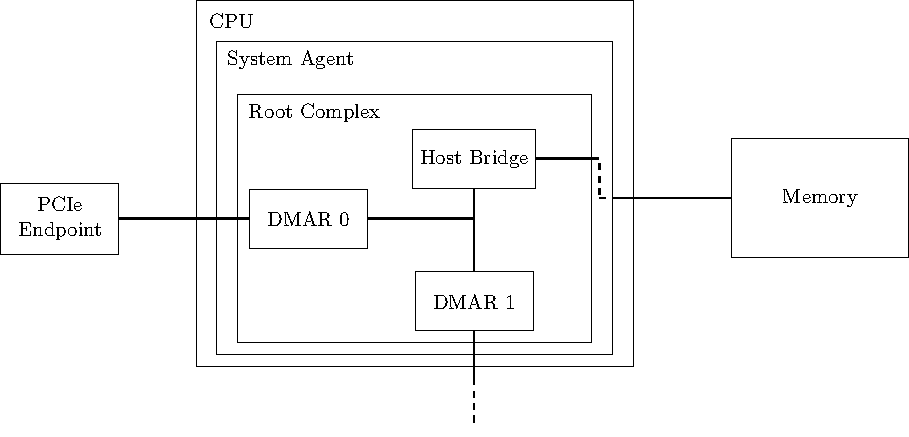
\includegraphics[width=0.7\textwidth]{figures/pcie-dmar}
    \caption{DMAR units in the PCIe root complex of an Intel system.}
    \label{fig:pcie-dmar}
\end{figure}

Every \ac{pcie} root complex may contain one or multiple \acp{iommu} where each
\ac{dmar} unit is responsible for a distinct set of \ac{io} buses
(\Cref{fig:pcie-dmar}). Devices on \ac{iommu}-managed buses belong to protection
domains, i.e., sets of address mappings and access permissions. While domains
may consist of multiple devices, devices belong to exactly one domain.

Data structures used for address translation by \ac{dmar} units are kept in main
memory to be accessible for \ac{os} and \acp{iommu}. In case of multiple
\acp{iommu}, \ac{dmar} units may share the same data structures. On \ac{iommu}
initialization, the \ac{os} sets up these data structures by creating domains
and address mappings for the system's \ac{io} devices. Although this happens at
system boot, mappings are not fix: the device-to-domain mapping may change
(e.g., when a device is assigned to a virtual machine) and address mappings may
be altered by the \ac{os} (e.g., when \ac{dma} memory is mapped or unmapped).

When \ac{io} devices attempt to access main memory, the request is intercepted
by the \ac{dmar} unit, checked for admissibility and translated appropriately.
This procedure consists of two major steps: First, a device's domain is
determined by its \ac{bdf} number. Second, the domain's translation tables are
consulted to map the requested address to the host physical address, taking into
account the domain's translation scheme. Depending on the usage model of the
\ac{iommu}, the addresses used by \ac{io} devices may be one of the following:

\begin{itemize}
    \item \acp{iova} managed by software on the host,
    \item guest \acp{iova} managed by software in a virtual machine,
    \item guest physical addresses of a virtual machine,
    \item guest virtual addresses of software running in a virtual machine.
\end{itemize}

\begin{figure}[!b]
    \centering
    \includegraphics[width=1.0\textwidth]{figures/iova-translation}
    \caption{Intel \acs{iommu} address translation of 48-bit addresses to 4~KiB
    pages. Adapted from \cite{morgan2018iommu}.}
    \label{fig:translation}
\end{figure}

For different address types, hardware implementations of \acp{iommu} may support
different translation schemes. In case of virtualization, \acp{iommu} may be
used for nested translation of addresses: a first-level translation to translate
a guest virtual address to a guest physical address, followed by a second-level
translation translating the guest physical address to the host physical address.

\Cref{fig:translation} depicts the address translation mechanism of an Intel
\ac{iommu} for 48-bit \acp{iova} to 4 KiB pages. After an attempt to read or
write main memory has been intercepted by the \ac{iommu}, the first table to be
consulted -- if translation was enabled in the global command register of the
\ac{iommu} -- is the root table. The physical address of the root table is
stored in the Root Table Address Register (RTAR) of the \ac{iommu}. The root
table consists of 256 root entries \SI{16}{\byte} each, i.e., \SI{4}{\kibi\byte}
in total. Every root entry has a bit that indicates presence of a context table
for this entry. The root table is indexed by the bus number of the device and --
in conjunction with device and function number -- determines the context entry
for this device.

Like the root table, the context table is a \SI{4}{\kibi\byte} page with 256
\SI{16}{\byte} entries. Every context entry represents an \ac{iommu} domain.
Context entries contain a field indicating whether requests belonging to this
domain may pass the \ac{iommu} untranslated, and -- in the more likely case that
addresses must be translated -- a pointer to the first table to be used for
address translation for this domain, the PML4 table.

Subsequently, PML4, PDP, PD and the page table are walked by the \ac{iommu} to
determine the host physical address belonging to the \ac{iova}. Every table is a
\SI{4}{\kibi\byte} page with 512 \SI{8}{\byte} entries. If there is no
translation for a requested address or the access rights for the associated page
do not permit access, translation faults and the request is rejected.

In case of \SI{2}{\mebi\byte} pages, no PT table is used for translation, and
the last \SI{21}{\bit} of the \ac{iova} represent the offset into the
\SI{2}{\mebi\byte} page. In case of \SI{1}{\gibi\byte} pages, no PT and no PD
table are used, and the last \SI{30}{\bit} of the \ac{iova} represent the offset
into the \SI{1}{\gibi\byte} page. PML4, PDP, PD and PT table form a 4-level
translation structure. For 57-bit \acp{iova} and \SI{4}{\kibi\byte} pages, a
5-level structure is used with an additional PML5 table. For 39-bit \acp{iova}
and \SI{4}{\kibi\byte} pages, only three tables are used.

Intel's \ac{iommu} uses two different formats for the page table entries. For
first-level translation, entries equal the format used by the \ac{mmu} such that
the \ac{cpu} page tables can be re-used for address translation. For
second-level translation, a unique format is used.

AMD's \ac{iommu} is mostly identical to Intel's. One of the major differences is
that the AMD \ac{iommu} uses one table (called device table) to determine the
\ac{iommu} domain from the \ac{pcie} \ac{bdf} identifier while Intel uses two,
root table and context table. With 65,536 possible \ac{bdf} combinations, AMD's
device table consists of up to 65,536 entries with \SI{256}{\bit} each, i.e., up
to \SI{2}{\mebi\byte}. Another difference of AMD's \ac{iommu} is consistent
usage of the \ac{mmu} page table entries format for all translations.

ARM on the other hand uses a completely different design for its \ac{iommu}. Its
SMMUv2 specification describes a register-based architecture for small-scale
systems, and SMMUv3 with \ac{iommu} configuration stored in memory for larger
systems. The translation tables of these \acp{iommu} are compatible to the ARMv8
architecture. Like AMD's and Intel's \ac{iommu}, ARM determines the context of
the supplied address before address translation, however, context does not
depend on the \ac{bdf} but a stream ID that is transmitted with every memory
transaction.

Common to all \acp{iommu} is caching of translation information in a context
cache and a \ac{tlb}, the \ac{iotlb}, to speed up address translation. While
context cache and \ac{iotlb} increase performance, they also increase complexity
as caches have to be kept up-to-date and entries must be purged from the caches
when they become invalid. If not implemented properly, this creates new
vulnerabilities as previous attacks have shown.


\section{IOMMUs on Linux}
\label{sec:iommus_on_linux}

Linux supports \acp{iommu} of all major vendors: besides Intel and AMD, the
kernel also includes drivers for \acp{iommu} from ARM, Qualcomm, Texas
Instruments, Samsung, Nvidia, IBM and other, less well-known manufacturers.

\acp{iommu} are not used by default on all architectures. In case of Intel x86,
Linux ignores any \ac{dmar} units and enables its own software \ac{iommu} called
SWIOTLB. The SWIOTLB is a poor man's \ac{iommu} that uses bounce buffers: At
boot time, a contiguous chunk of memory (usually \SI{64}{\mebi\byte}) is
reserved in the lower address space of main memory and used for \ac{dma}-capable
devices with limited addressing capabilities, e.g., legacy 32-bit devices. When
an already allocated \ac{dma} buffer is to be used by a device that cannot
address the buffer directly, memory in the lower address space, the so-called
aperture, is linked to that buffer, passed to the device, and data is copied
back and forth by the \ac{os} between the device-used memory in the aperture and
the device-inaccessible buffer.

On AMD systems, \acp{iommu} are enabled by default. For Intel, this behavior can
be enforced through a kernel boot parameter. When \acp{iommu} are enabled, Linux
checks the \acs{acpi} tables of \ac{bios}/\ac{uefi} for \ac{dmar} units on
system boot. For every DMA Remapping Hardware Unit Definition (DRHD) in the
\ac{dmar} reporting \ac{acpi} tables, Linux initializes the \ac{dmar} unit
through its respective device driver, creates a default \ac{iommu} domain and
assigns all \ac{pcie} devices to \ac{iommu} groups, where each group represents
the smallest possible set of devices that can be distinguished by the \ac{iommu}
(e.g., all devices behind a \ac{pcie}-to-PCI bridge belong to the same group).
Furthermore, each \ac{iommu} group is assigned to an \ac{iommu} domain.

Linux has a number of kernel boot parameters to change its default behavior in
relation to \acp{iommu}. (SW-)\acp{iommu} can be disabled or enforced, the
default domain can be set to pass-through such that devices bypass the
\ac{iommu} if not specified otherwise, and depending on the driver, the policy
of \ac{iotlb} management can be changed as Linux defers \ac{iotlb} invalidation
by default which increases performance but creates a window for invalid \ac{dma}
accesses, i.e., devices may access some \ac{dma}-able memory that has been
unmapped already as requests are still translated by the \ac{iotlb}. For the
Intel \ac{iommu}, \ac{iotlb} invalidation can be set to strict mode to enforce
immediate flushing of the \ac{iotlb}. The AMD \ac{iommu} driver provides a
similar option called \texttt{fullflush}. If no deviating behavior is specified,
Linux flushes the \acp{iotlb} every \SI{10}{\ms} or every 256 batched
invalidation requests.

Device drivers do not configure \acp{iommu} directly. Instead, they change the
\ac{iommu} configuration through Linux's \ac{dma}-API by allocating, mapping and
unmapping \ac{dma} memory, enforcing action by the respective \ac{iommu}
driver(s) depending on the operation and settings (e.g., immediate flushing of
all \acp{iotlb}).

\ac{dma}-mapping functions of the kernel return physical addresses as \ac{dma}
address when the \ac{pcie} device uses no \ac{iommu} and \acp{iova} with
\ac{iommu}. In both cases, memory is allocated using one of the kernel memory
allocator functions. Only in the second case, however, an \ac{iova} from the
device \ac{iommu} domain is allocated and the mapping from \ac{iova} to physical
address of the allocated memory is created through the \ac{iommu} driver.

For each \ac{iommu} domain, a base address and the upper boundary of
device-addressable \acp{iova} are assigned on initialization. Allocated
\acp{iova} are stored in a red-black tree which on allocation is searched for a
fitting address range bottom-up, i.e., from the highest \ac{iova} to the lowest.
To speed up \ac{iova} allocation, magazines are used, i.e., per core caches for
previously deallocated \acp{iova}.

For controlled device access in user space, e.g., by user space network drivers,
Linux offers a framework called \ac{vfio}. The framework consists of a device
driver and various \texttt{ioctl}s to interact with \ac{iommu}-controlled
\ac{pcie} devices.

Devices to be used through \ac{vfio} have to be bound to the \ac{vfio} device
driver. If a device's group contains multiple devices, all have to be bound to
the driver or must be unbound from other host drivers (which will make the group
available except the unbound devices). Device groups successfully bound to the
\ac{vfio} driver appear as files in Linux's device filesystem at
\texttt{/dev/vfio/\{group-number\}}. By chowning a device's group file to the
current user, unprivileged access to the \ac{pcie} devices of the group is
granted in a safe manner.

In \ac{vfio}, every \ac{iommu} group in use belongs to a container. Depending on
the \ac{iommu} driver's capabilities, one or multiple groups may be encapsulated
into a container, and containers may contain groups of different \ac{iommu}
domains.

To access a \ac{vfio}-bound device in user space, multiple steps have to be
carried out by an application. The steps follow this scheme: First, a \ac{vfio}
container is created and initialized for the device to be used or an existing
container is re-used. Second, the device's group file is opened by the
user space application and the group is added to the \ac{vfio} container. Third,
a file descriptor to the device is derived through a \ac{vfio} \texttt{ioctl}
call on the group file. Fourth, the device file descriptor is used to map the
device's registers into virtual memory. Finally, memory for \ac{dma} operations
may be allocated in user space and \ac{iommu} mappings to that memory may be
created through the \ac{vfio}-API, returning \acp{iova} that can be passed to
the device.

Internally, \ac{vfio} stores its \ac{iova} mappings in a red-black tree.
Multiple mappings may be coalesced to reduce tracking overhead. When a new
mapping is requested through the \ac{vfio}-API, the red-black tree is checked
for overlapping mappings, validity of the requested \ac{iova} range is verified
(e.g., supported address width by affected \acp{iommu} vs. provided \ac{iova}
address width), the mapping is inserted into the tree, pages are pinned for
\ac{dma} access and the mapping is created in the \ac{iommu} tables via the
kernel-internal \ac{iommu}-API.


\section{Single-Root Input/Output Virtualization}
\label{sec:sriov}

% TODO: image physical function vs virtual function?

\Acf{sriov} is a mechanism that allows \ac{pcie} devices to appear as multiple
devices and thus be shared with multiple virtual machines. Devices that support
\ac{sriov} report this ability to the host via their PCI configuration space
which includes registers for \ac{sriov} Extended Capability.

When \ac{sriov} is enabled for a device, the device can be split into a \ac{pf}
and multiple \acp{vf}. The \ac{pf} is the standard \ac{pcie} function of the
device which has full control over the device, is used to reset and initialize
it and to enable and disable \acp{vf}. Hence, access to the \ac{pf} is usually
restricted to \ac{os} or virtual machine manager (VMM). \acp{vf} on the other
hand only support a subset of device operations, primarily to manage packet
receival and transmittal of the function, and can be passed to virtual machines
in a safe manner.

For \acp{vf}, separate drivers are used as \acp{vf} use different device
registers and have to communicate with the \ac{pf} driver for certain operations
like reset of the \ac{vf}. A \ac{pf} driver on the other hand must be able to
handle these requests and is hence slightly more complex than the same driver
without \ac{sriov} support.

On Linux, \acp{vf} of \ac{sriov}-capable devices can be created when loading the
\ac{pf} kernel driver, e.g., in case of \texttt{ixgbe}: \texttt{modprobe ixgbe
max\_vfs=2}, which results in the \ac{pf} driver creating two \acp{vf} for every
\texttt{ixgbe}-bound device in the system, or by writing the required number of
\acp{vf} into a device \texttt{sysfs} file called \texttt{sriov\_numvfs}.

When \acp{vf} are created by the \ac{pf} driver, every \ac{vf} is assigned a
\ac{pcie} \ac{bdf} triple such that the \ac{vf} can be identified on the
\ac{pcie} bus and adressed directly. Although the function part of the \ac{bdf}
is only \SI{3}{\bit}, i.e., eight different functions, more \acp{vf} can be
created by using different device numbers for the \acp{vf}.

Usually, the \ac{pf} also assigns \ac{mac} addresses to the \acp{vf} and
configures the \ac{nic} such that each \ac{vf} receives the packets destined to
its \ac{mac} address. To prevent \ac{mac} address spoofing, outgoing packets
must be sent from the \ac{vf}'s \ac{mac} address and are dropped by the \ac{nic}
in case \acp{vf} do not comply. The \ac{mac} anti-spoofing mechanism can be
disabled by the \ac{pf} driver.

While not required, \ac{sriov} can be used in conjunction with \acp{iommu} to
pass \acp{vf} safely to virtual machines. When devices are passed-through
without \acp{iommu}, virtual machines have unlimited access to the machine's
main memory through the virtual function (see \Cref{sec:dma}).



\chapter{Related Work}
\label{chap:related_work}

Publications on \acp{iommu} can be split into four categories:
(1)~basic documentation and evaluation of \ac{iommu} utilization in Linux and
   Xen,
(2)~performance analyses of \acp{iommu},
(3)~\ac{iommu} emulation and usage in the context of virtualization, and
(4)~\ac{os} vulnerabilities by incorrect use of \acp{iommu}.

Early papers covered Sun Microsystem's \ac{iommu} on SPARC stations of the Sun-4
architecture which was launched in 1987 \cite{miller1996linux,
kunisawa1997gigabit}.
Miller and de Icaza documented their efforts to port Linux to the SPARC
platform, describing implementation hurdles and differences between various
versions of the Sun-4 architecture \cite{miller1996linux}. They note that on
larger machines the Sun \ac{iommu} forms a separate \ac{mmu} on the chipset,
whereas on smaller machines it is included in the processor.

In 2006, research shifted to the previously released \acp{iommu} from Intel, AMD
and IBM that marked a paradigm change: While former \acp{iommu} had been
primarily used for address translation to enable \ac{dma} devices to access all
physical memory of a host, these new \acp{iommu} were also capable of device
isolation, i.e. restricting memory access of devices to device-specific memory
regions \cite{ben2006utilizing}. Performance evaluations of these \acp{iommu}
focused on \ac{cpu} load: Ben-Yehuda et al. claim that IBM's Calgary/DART
\acp{iommu} do not affect \ac{io} throughput, however, \ac{cpu} utilization
increases by up to 60\% in some scenarios \cite{ben2007price}. They identify
\ac{iova} (de-)allocation as the primary factor of high \ac{cpu} load and thus
propose batching memory map and unmap calls or eliminating them wherever
possible.

Later scientific work revealed more bottlenecks in hardware and software. Amit
et al. focus on the \ac{iommu} \ac{iotlb} \cite{amit2010iommu}. They note that
the \ac{tlb} of their Intel Xeon X5570 \ac{iommu} gets thrashed when more than
16 pages are used, increasing \ac{cpu} execution time by up to 47\%. To evaluate
different replacement strategies for \ac{iotlb} entries, they implement a
virtual \ac{iommu} for the KVM hypervisor which lets them trace map/unmap
operations and analyse \ac{io} memory access patterns. Based on their results,
they propose changes in software and hardware that can reduce \ac{iotlb} misses
by over 60\%.

In a follow-up paper \cite{amit2011viommu}, Amit et al. use their virtual
\ac{iommu} to investigate different mapping strategies and performance/security
implications of delayed \ac{iotlb} invalidations. They conclude that delaying
\ac{iommu} unmappings for a few milliseconds can lead to a significantly higher
througput if \ac{dma} buffers are reused often (and are consequently not
unmapped and invalidated in the \ac{iotlb}).

For devices with ring buffers, Malka et al. propose a new \ac{iommu} design with
drastically reduced overhead for \ac{iova} (de-)allocation and a one-entry
\ac{iotlb} per memory ring \cite{malka2015riommu} to keep up with the increasing
speeds of \ac{io} peripherals.

Peleg et al. take a look at concurrent \ac{iova} assignment and \ac{iotlb}
management for scalable use of \acp{iommu} \cite{peleg2015utilizing}. They
propose three designs for \ac{iova} assignment and a new \ac{iotlb} invalidation
scheme.


Other researchers focus on security. Markettos et al. investigate the handling
of \acp{iommu} by \aclp{os} \cite{markettos2019thunderclap}. They build their
own FPGA platform to attack systems as malicious Thunderbolt peripherals, and
discover eight major vulnerabilities in Windows, Linux and macOS.



\chapter{Implementations}
\label{chap:implementations}

To analyse performance, safety and security implications of \acp{iommu}, we use
\texttt{ixy.rs} \cite{ellmann2018writing}, a high-speed user space network
driver written in Rust for Intel 10G \acp{nic} of the \texttt{ixgbe} family, and
adapt it to our needs. Changes to the existing implementation and new code are
described in the following sections. All architectural and \ac{os}-related
remarks refer to Linux on x86-64, the target platform of \texttt{ixy.rs}.


\section{ixy.rs}
\label{sec:ixy_rs}

Stefan Huber added basic \ac{iommu} support to \texttt{ixy.rs} in 2019 through
Linux's \ac{vfio} API \cite{huber2019using}. We complete the implementation by
adding support for the following two use cases: accessing multiple devices
associated to the same \ac{iommu} group and using \texttt{ixy.rs} in conjunction
with legacy \acp{iommu} not supporting 48-bit wide \acp{iova} for second-level
address translation (i.e., the translation mode used by \ac{vfio}).

For the former, only minor changes in the code are necessary. In the original
implementation, a device's \ac{vfio} group file is opened on device setup and
closed after the \ac{vfio} device file descriptor was derived from the group.
However, a device group file cannot be re-opened if it is used through a derived
device file descriptor, even if the descriptor of the group file was properly
closed. Re-opening the group file in that case returns \ac{os} error 16, i.e.,
``device or resource busy''. We mitigate this problem by keeping \ac{vfio} group
files opened and storing the file descriptors in a \texttt{HashMap<i32, RawFd>}
that maps \ac{iommu} groups to group file descriptors. When a new device is
initialized, the \texttt{HashMap} is checked for the \ac{vfio} group. In case
there is no key-value pair for the group, the group file is opened and group
number and descriptor are added to the \texttt{HashMap}. Otherwise, the group
file descriptor from the \texttt{HashMap} is used.

To use \texttt{ixy.rs} with \acp{iommu} with a maximum second-level translation
\ac{iova} widths smaller than the host's virtual address widths (e.g., only 39
instead of \SI{48}{\bit}), we reduce the \ac{iova} widths in \texttt{ixy.rs}.
Currently, \texttt{ixy.rs} uses a 1:1 mapping of process virtual addresses to
\acp{iova} when setting up the \acp{dmar}. Hence, \ac{mmu} and \ac{iommu} map
the same (\ac{io}) virtual addresses to the same physical addresses and there is
no need for \texttt{ixy.rs} to track which \ac{iova} is used for which \ac{dma}
buffer. We keep this mapping for simplicity but enforce all memory to be used by
the \ac{nic} to be mapped into the lower \SI{32}{\bit} of the process address
space. To our knowledge, there are no \acp{iommu} for the x86 architecture that
do not support addresses up to \SI{39}{\bit}.

On a side note: a 1:1 mapping of process virtual addresses to \acp{iova} is one
of the use cases mentioned in Intel's \ac{iommu} specification as Shared Virtual
Memory (SVM) \cite[p.~21]{intel2019iommu}. Unfortunately, we cannot make use of
SVM since neither the \texttt{ixgbe} \acp{nic} nor Linux's \ac{vfio} framework
support the required \ac{pcie} feature (PASID). In general, PASID seems to be a
rather rare feature: Rothwell states in his dissertation that he has not seen it
used in practice \cite[p.~31]{rothwell2018exploitation}.

Mapping memory into the 32-bit address space of a process is not rocket science.
\texttt{mmap} can be forced through the \texttt{MAP\_32BIT} flag to create
mappings in the first \SI{4}{\gibi\byte} of the process address space (indeed,
only \SI{2}{\gibi\byte} are used, which is why some authors call it the
\texttt{MAP\_31BIT} flag). However, mapping memory gets more sophisticated when
huge pages are used (as they are in \texttt{ixy.rs}) due to alignment
requirements: huge pages have to be huge-page-aligned, i.e., at
\SI{2}{\mebi\byte} or \SI{1}{\gibi\byte} boundaries. Due to the alignment
requirements, calling \texttt{mmap} with \texttt{MAP\_32BIT} and
\texttt{MAP\_HUGETLB} fails.

To obey the alignment, we use \texttt{mmap} twice: to determine an appropriate
address range and to map the huge pages into the address range.
\Cref{lst:32-bit-map} illustrates the algorithm. First, a mapping of needed size
plus one huge page size is created (where needed size is equivalent to one or
multiple huge pages). We know that any address range of size $s$ contains a
$s$-aligned address, i.e., for any address $r$ returned by \texttt{mmap} we know
that ${\exists a \in \{r, r + 1, ..., r + s - 1\}: a \equiv 0 \mod s}$. Thus we
use the additionally mapped huge page to find the huge-page-aligned address $a$.
After that, excess memory is freed, i.e., memory between the \texttt{mmap}-
returned address and the huge-page-aligned address and any remaining bytes of
the additionaly mapped huge page at the end of the mapping. Finally, huge pages
of the needed size are mapped to the huge-page-aligned address by a second call
to \texttt{mmap}, passing the aligned address as first argument to \texttt{mmap}
and the flag \texttt{MAP\_FIXED} to force \texttt{mmap} to map the huge pages at
the specified address.

\begin{minipage}{\textwidth}
    \lstinputlisting[label={lst:32-bit-map},language=Rust,caption={Mapping huge
    pages into the first \SI{2}{\gibi\byte} of the process address space.},
    captionpos=b]{code/32-bit-map.rs}
\end{minipage}

Besides these newly implemented features in \texttt{ixy.rs}, some minor changes
were made to the source code. We fixed a bug in the memory module where virtual
addresses where used instead of \ac{io} virtual addresses, a wrong bitmask was
discovered and corrected in the original ixy driver \cite{emmerich2019user} that
propagated into all re-implementations \cite{emmerich2019case} of the driver,
and some comments were updated, typos fixed and overall code cleanliness
improved (removal of superfluous casts, parentheses, etc.).


\section{ixgbevf}
\label{sec:ixgbevf}

To analyse the effects of \acp{iommu} in context of \ac{sriov}, we implement
\texttt{ixgbevf} for \texttt{ixy.rs}, a variant of the \texttt{ixgbe} driver for
\ac{sriov} \acp{vf}. We base our implementation on the \texttt{ixgbevf} code in
the Linux kernel and DPDK, and the Intel 82599 SR-IOV Companion Guide
\cite{intel201082599}.

While \texttt{ixgbe} (\ac{pf} driver) and \texttt{ixgbevf} (\ac{vf} driver)
share large parts of their code base, device setup and communication between
driver and \ac{nic} differ, and there are some tasks on \acp{vf} (like reset)
that have to be executed cooperatively by both drivers. Besides these
differences in the drivers, there are also differences in the devices: \acp{vf}
support only up to 8 RX/TX queues in contrast to 64 of the \ac{pf}, and the PCI
configuration space of \acp{vf} returns \texttt{0xffff} for vendor and device
ID, making it necessary to grab the values from files in the \texttt{sysfs} or
from the \acp{pf}' PCI configuration spaces to determine the correct driver to
be used.

Reset and initialization of the \ac{pf}, i.e., the device itself, and creation
of \acp{vf} is initiated by the \ac{pf} driver. The \ac{pf} driver brings the
\ac{nic} into an operational state and creates \acp{vf} when requested to do so,
e.g., by the \ac{os}.

Reset and initialization of the \ac{vf} is initiated by the \ac{vf} driver. To
reset the \ac{vf}, communication with the \ac{pf} driver is necessary. In
general, \ac{vf} driver communication happens in two ways: Directly with the
\ac{nic} via memory-mapped \ac{io} and by passing messages to the \ac{pf} driver
via a mailbox system. For direct communication with the \ac{nic}, only a part of
the device configuration space can be accessed by the \ac{vf}.  The registers in
this configuration space allow the \ac{vf} driver to set up the descriptor
rings, enable or disable interrupts, send and receive packets, etc.  For
operations that have global impact like configuring VLAN filters or resetting
the \ac{vf}, the \ac{vf} driver has to communicate with the \ac{pf} driver and
request the needed operations. This is done via a mailbox system that is
implemented in hardware in the \ac{nic}.

Messages used for mailbox communication are hardware-independent and can be
freely chosen by driver implementations. However, to be able to use our driver
in conjunction with the kernel \texttt{ixgbe} driver as \ac{pf} driver, we have
to use the same messages for the same operations. Hence, we implement the
mailbox in the way the Linux kernel driver and DPDK do.

\Cref{lst:mbx} shows how communication with the \ac{nic} mailbox is implemented
in \texttt{ixgbevf}. \linebreak \texttt{read\_msg\_from\_mbx} is used to read a
message from the mailbox buffer. It is expected to be called once a new message
for the \ac{vf} arrives (which can be determined through the
\texttt{IXGBE\_VFMAILBOX} register). The method takes a slice \texttt{msg} of
unknown size to store the message from the mailbox. Before the message is copied
to the slice, the mailbox is locked to prevent race conditions between \ac{vf}
and \ac{pf}. Subsequently, the message is copied and receipt of the message
acknowledged (releasing the mailbox at the same time).

\begin{minipage}{\textwidth}
    \lstinputlisting[label={lst:mbx},language=Rust,caption={Reading a message
    from the VF mailbox.},captionpos=b] {code/mbx.rs}
\end{minipage}

\ac{vf} initialization of \texttt{ixgbevf} resembles to a large extent \ac{pf}
initialization of \texttt{ixgbe}: Once the \ac{vf}'s registers are mapped into
memory and \ac{dma} bus master is enabled for the \ac{vf}, interrupts are
disabled and the \ac{vf} is reset by prompting the \ac{pf} driver for function
reset. When the \ac{pf} driver has acknowledged function reset, the \ac{mac}
address of the \ac{vf} is derived from the \ac{pf} through mailbox communication
or generated locally. Subsequently, RX and TX descriptor rings are set up and
initialization of the \ac{vf} is complete.

Unlike in \texttt{ixgbe}, there is no link setup since the \ac{pf} driver is
responsible for the link. Indeed, \acp{vf} can only be used once the device's
link is up. If the link is down, \ac{vf} reset stalls. If the link goes down
while \acp{vf} are used, the \acp{vf} become inoperable and have to be reset
once the \ac{pf}'s link is up again.

Deriving the \ac{mac} address and using it as source address for outgoing
packets is crucial for \texttt{ixgbevf} as the kernel driver enables \ac{mac}
anti-spoofing by default, i.e., all TX packets are checked for deviating
\ac{mac} addresses by the \ac{nic} and get discarded if a deviating address was
detected.


\section{iommu-leaks}
\label{sec:iommu_leaks}

For precise time measurements on \ac{nic} operations and to analyse effects of
the \ac{iotlb}, we implement some additional functionality in \texttt{ixy.rs}.

To be independent of the physical link, we add methods to enable loopback
operations on the \ac{nic}. In loopback mode, packets are transmitted from the
\ac{nic}'s TX queues via its internal 10 Gigabit Media Independent Interface
(XGMII) to the RX queues without leaving the device.

We also add methods to dynamically enable and disable queues. This is
advantageous to approximate how much time is needed for \ac{dma} transfers. By
disabling all RX queues, TX transmit times can be broken down to a \ac{dma}
access to the TX queue page and another \ac{dma} access to the packet buffer.

To measure \ac{cpu} cycles for \ac{nic} operations, we use the x86
\texttt{rdtsc} instruction. We implement a rdtsc function as shown in
\Cref{lst:rdtsc}. We use intrinsic functions to avoid inline assembler. Since
intrinsic functions are inherently unsafe, we need an \texttt{unsafe} block.
Note our use of memory fences to serialize instruction execution.
\texttt{lfence}s deter the compiler from reordering code and the \ac{cpu} from
speculatively executing subsequent instructions, namely the \texttt{rdtsc}
itself and following instructions. Unlike suggested by a Intel in a benchmarking
guide for the IA-32 and IA-64 architecture \cite{paoloni2010benchmark}, we use
\texttt{lfence} instead of \texttt{cpuid} as it provides the same serialization
guarantees and keeps the variance small.

\begin{minipage}{\textwidth}
    \lstinputlisting[label={lst:rdtsc},language=Rust,caption={\texttt{rdtsc()}
        function to count \acs{cpu} cycles.},captionpos=b]
        {code/rdtsc.rs}
\end{minipage}

To be able to evaluate measured \ac{cpu} cycles, we implement a logger that logs
values to a file-backed huge page and provides statistics about the measured
values like mean, variance and sample variance.

For \ac{iotlb}-related research, we implement a brute-force memory allocator
that allocates physically and virtually contiguous 4 KiB pages. By using normal
sized pages, locality of packet buffers can be maintained while the amount of
pages to be translated by the \ac{iommu} respectively the \ac{iotlb} can be
controlled variably.

The memory allocator works as follows: First, two memory regions are allocated
via \texttt{mmap}, a huge region -- which is our page pool -- containing 1,024
pages that are checked for contiguity and a target memory area. Next, virtual
and physical address of every page in the page pool are inserted into some data
structure, e.g., a vector, and sorted by ascending physical addresses.
Subsequently, the sorted pages are remapped to the target memory area using
\texttt{mremap} and checked for contiguity. Since all pages have been remapped
in physically contiguous order, physically adjacent pages are now also adjacent
in virtual address space. Thus, it suffices to iterate through the target memory
area and check whether there is a block of physically subsequent pages big
enough to satisfy the requested amount of contiguous memory.

To control memory placement of RX/TX queues and packet buffers, we add methods
to \texttt{ixy.rs} that reinitialize the aforementioned data structures at
variable memory addresses, e.g., memory allocated by our brute-force memory
allocator. We also add methods for fine-grained control of TX descriptors and
queues that allow us to repeatedly use the same descriptor(s) for transmit.



\chapter{Performance Analysis}
\label{chap:performance_analysis}

To determine the performance impact of \acp{iommu} on throughput and latency, we
conduct various measurements using the implementations described in
\Cref{chap:implementations}, i.e., \texttt{ixy.rs}, \texttt{ixgbevf} and
\texttt{iommu-leaks}.


\section{Methodology}
\label{sec:methodology}

% TODO: illustration of test setup?

\begin{table}
    \centering
    \begin{tabular}{lllrll}
        \textbf{CPU} & \textbf{Year} & \textbf{Arch.} & \textbf{Memory} & \textbf{NIC} & \textbf{NUMA} \\
        \toprule

        \multirow{2}{*}{Intel Xeon E3-1230v2} & \multirow{2}{*}{2012} &
        \multirow{2}{*}{Ivy Bridge} & \multirow{2}{*}{\SI{16}{\giga\byte}} & Intel X520-DA1 &
        \multirow{2}{*}{no} \\
        & & & & Intel X520-DA2 & \\ \hline

        \multirow{2}{*}{Intel Xeon E5-2620v3} & \multirow{2}{*}{2014} &
        \multirow{2}{*}{Haswell} & \multirow{2}{*}{\SI{32}{\giga\byte}} & Intel X520-DA2 &
        \multirow{2}{*}{no} \\
        & & & & Intel X540-T2 & \\ \hline

        \multirow{2}{*}{AMD EPYC 7551P} & \multirow{2}{*}{2017} &
        \multirow{2}{*}{Naples} & \multirow{2}{*}{\SI{128}{\giga\byte}} & Intel X550T &
        \multirow{2}{*}{yes} \\
        & & & & Intel X550T & \\

        \bottomrule
    \end{tabular}

    \caption{System configurations of servers used for performance analysis.}
    \label{tab:servers}
\end{table}

All measurements are performed on server pairs connected via two 10 Gbit/s
links. The devices under test use Intel \acp{nic} of the \texttt{ixgbe} family
that are compatible with our drivers, i.e., X520, X540 and X550. Each device
under test is equipped with two of these cards since two separate \acp{nic}
yield better performance than a dual-ported one (probably due to hardware
limitations of the \ac{pcie} connection). \Cref{tab:servers} lists the devices
under test.

On the devices under test, we run the different implementations. For the
measurements, two applications are used on top of the drivers, a traffic
generator and a forwarder. The traffic generator allocates a memory pool and
repeatedly sends out the same buffers, only updating the sequence numbers of the
packets. The forwarder uses two devices, allocates a pool per device and
forwards packets bidirectionally, i.e., packets received by the first device are
sent out by the second and vice-versa. To simulate a somewhat realistic
workload, one byte of each packet is increased, enforcing the \ac{cpu} to load
the byte into the \ac{cpu} caches. On the second server, MoonGen
\cite{emmerich2015moongen} generates traffic with its
\texttt{l2-load-latency.lua} script.

All benchmarks are conducted at native \ac{cpu} frequency with dynamic
overclocking disabled. \ac{cpu} cores are pinned for the measurements. On NUMA
architectures, i.e., the AMD server, locality is obeyed for \ac{cpu} core
pinning and memory placement. \Cref{tab:cpus} contains details of the \acp{cpu}.
Two important characteristics emerge from the table: clockspeed has a huge
impact on single thread/core performance while the absolute number of cores is
crucial for overall \ac{cpu} performance.

Our benchmarking applications are executed on a single \ac{cpu} core in a single
thread as full support for multi-core systems is not implemented in the drivers
yet. On most systems this is not a limitation as hardware limits can be hit with
a single thread. It stands out from \Cref{tab:cpus} that -- although being the
oldest of the three \acp{cpu} -- the Intel Xeon E3 yields the highest per-thread
performance while the AMD \ac{cpu} performs worst. This observation is backed by
our baseline measurements (\Cref{sec:baseline_measurements}).

To reduce architecture-dependent overhead and assimilate the results of our
measurements, packet-prefetching is disabled in all implementations. If not
specified otherwise, packets are processed in batches of 32, ring sizes of 512
are used for RX and TX descriptors, and all \ac{dma}-able memory is allocated on
2 MiB huge pages. On RX overload, packets are dropped by the \ac{nic}.

Throughput and latency results of the implementations are measured on the second
server by MoonGen. Forwarded and generated packets contain 60~B of data, i.e.,
84~B with checksums and interpacket gap which is the minimum Ethernet frame
size, such that line rate at 14.88 Mpps can be achieved in all measurements.

\begin{table}
    \centering
    \begin{tabular}{llrrrr}
        \multirow{2}{*}{\textbf{CPU}} & \multirow{2}{*}{\textbf{Clock}} &
        \multirow{2}{*}{\textbf{Cores}} & \multirow{2}{*}{\textbf{L3-Cache}} &
        \multicolumn{2}{r}{\textbf{PassMark}} \\
        & & & & \textbf{ST} & \textbf{All} \\
        \toprule

        Intel Xeon E3-1230v2 & \SI{3.3}{\giga\Hz} &  4 &  \SI{8}{\mega\byte} & 1,996 &  6,192 \\
        Intel Xeon E5-2620v3 & \SI{2.4}{\giga\Hz} &  6 & \SI{15}{\mega\byte} & 1,700 &  7,979 \\
        AMD EPYC 7551P       & \SI{2.0}{\giga\Hz} & 32 & \SI{64}{\mega\byte} & 1,611 & 25,933 \\

        \bottomrule
    \end{tabular}

    \caption{\acsp{cpu} of devices under test and their PassMark scores for
    Single Thread (ST) and all cores.}
    \label{tab:cpus}
\end{table}

For measurements including an \ac{iommu}, pass-through mode is used for the
\ac{iommu} to reduce side effects from other \ac{io} devices on the host. All
measurements are conducted with Rust 1.50.0 on Debian Buster 10.6 with a Linux
4.19 kernel.


\section{Baseline Measurements}
\label{sec:baseline_measurements}

To determine the baseline performance of our devices under test, we run the
forwarder and the generator application in default configuration on all servers.
\Cref{fig:baseline-perf} shows the results. Since the generator application
generates traffic on a single port only, we run two instances on two different
devices for our measurements. Consequently, the bars on the left of
\Cref{fig:baseline-perf-throughput} show single core forwarding rate while the
bars on the right show dual core packet generation rate. Since the two instances
of the packet generator are executed independently of each other on two
different \ac{cpu} cores and devices, single core packet generation rate equals
(approximately) the measured results divided by two.

\begin{figure}%[!b]
	\centering
	\subfloat[Throughput]{%
        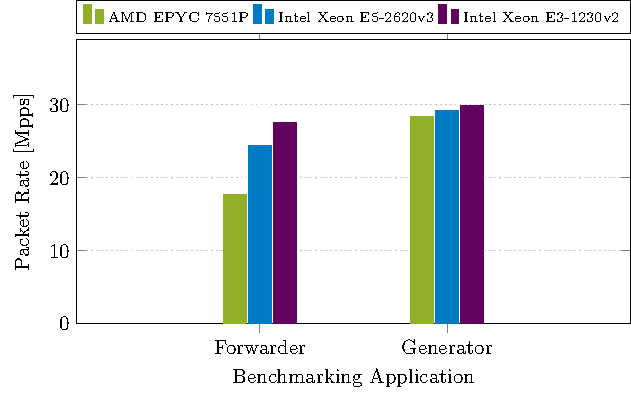
\includegraphics[width=0.46\textwidth]{figures/baseline-throughput}
		\label{fig:baseline-perf-throughput}
	}
	\subfloat[Latency]{%
        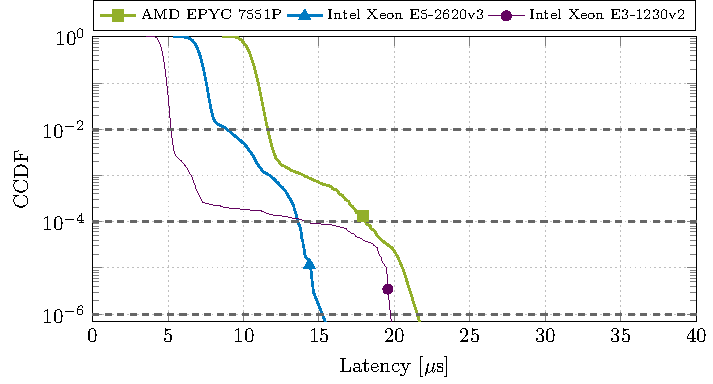
\includegraphics[width=0.54\textwidth]{figures/baseline-latency}
		\label{fig:baseline-perf-latency}
	}

    \caption{Baseline throughput and latency of servers used for performance
    measurements. Latency of forwarder measured with a total packet rate of 10
    Mpps.}
	\label{fig:baseline-perf}
\end{figure}

From \Cref{fig:baseline-perf-throughput}, it is particularly striking that the
packet forwarder on the AMD EPYC \ac{cpu} (packet rate: 17.6~Mpps) is about one
third slower than on the Intel Xeon E5 \ac{cpu} (packet rate: 24.4~Mpps)
although clockspeeds differ only by one sixth.

We use \ac{cpu} performance counters to profile the forwarder with both
\acp{cpu} and identify two reasons for the poor performance of the AMD \ac{cpu}:
the AMD \ac{cpu} executes about 1.75 instructions per cycle (IPC) while the
Intel \ac{cpu} runs about 2.1, and while 0.01-0.03\% of all branches are
mispredicted on the Intel \ac{cpu}, the AMD \ac{cpu} has a misprediction rate of
0.40\%.

Although AMD EPYC's Naples architecture is based on Zen, we find reports on poor
IPC counts and branch misses for the successor architecture of Zen -- Zen 2 --
which seem to support our findings \cite{lemire2019instructions,
lemire2019mispredictions}. Compared to Intel Skylake, the AMD Zen 2 \ac{cpu}
seems to take one to two additional cycles per branch misprediction.

Looking at \Cref{fig:baseline-perf-throughput}, both Intel \acp{cpu} stand out,
with the cheaper Xeon E3 \ac{cpu} introducing more variance into latency while
the more expensive Xeon E5 \ac{cpu} forwards traffic rather smoothly.


\section{Page Sizes}
\label{sec:page_sizes}

\begin{figure}[!b]
	\centering
	\subfloat[4 KiB pages, stack]{%
        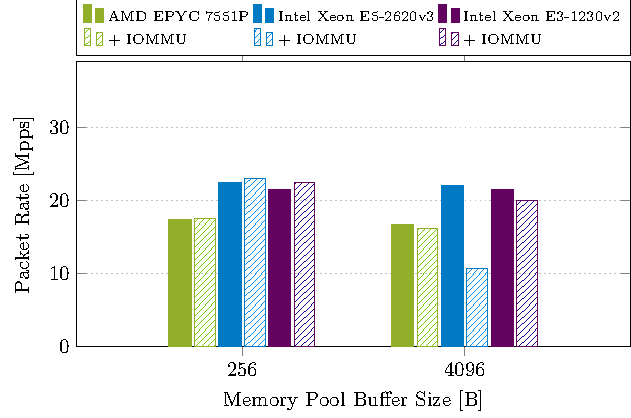
\includegraphics[width=0.46\textwidth]{figures/page-size-4k-throughput}
		\label{fig:page-size-4k-throughput}
	}
	\subfloat[4 KiB pages, queue]{%
        \includegraphics[width=0.46\textwidth]{figures/page-size-4k-queue-throughput}
		\label{fig:page-size-4k-queue-throughput}
	}
    \par
	\subfloat[2 MiB pages, stack]{%
        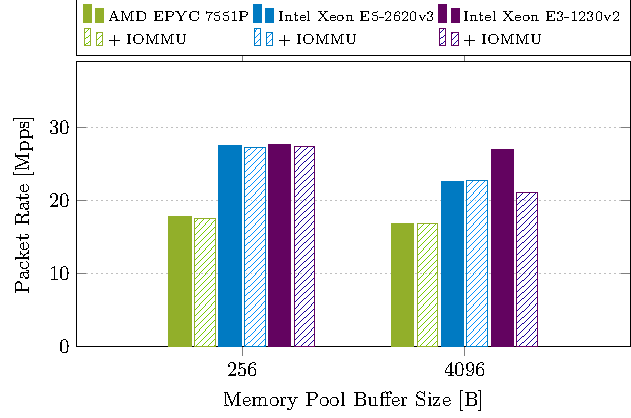
\includegraphics[width=0.46\textwidth]{figures/page-size-2m-throughput}
		\label{fig:page-size-2m-throughput}
	}
	\subfloat[2 MiB pages, queue]{%
        \includegraphics[width=0.46\textwidth]{figures/page-size-2m-queue-throughput}
		\label{fig:page-size-2m-queue-throughput}
	}
    \par
	\subfloat[1 GiB pages, stack]{%
        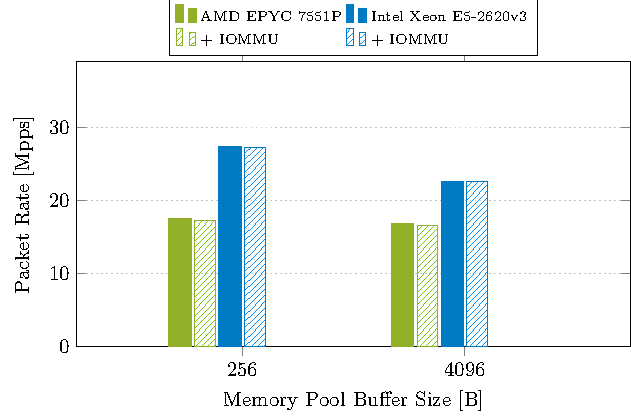
\includegraphics[width=0.46\textwidth]{figures/page-size-1g-throughput}
		\label{fig:page-size-1g-throughput}
	}
	\subfloat[1 GiB pages, queue]{%
        \includegraphics[width=0.46\textwidth]{figures/page-size-1g-queue-throughput}
		\label{fig:page-size-1g-queue-throughput}
	}

    \caption{Throughput of forwarder with different page sizes, memory pool
    buffer sizes and data structures for the memory pool.}
	\label{fig:page-size-throughput}
\end{figure}

It is well known that page sizes impact system performance. Page sizes are a
trade-off: When larger pages are used, overhead for page management decreases,
and page tables and the \ac{tlb} have to keep less entries. At the same time,
fragmentation and page swapping increases as even tiny amounts of data have to
be stored on whole pages and less pages can be kept in main memory at a time.
Smaller pages on the other hand increase page tables and put more pressure on
the \ac{tlb} since more pages have to be accessed for the same amount of data.
This can lead to \ac{tlb} thrashing: address translations are continuously
replaced by new translations in the \ac{tlb}, reducing effectiveness of the
cache. In extreme cases, addresses are re-translated for every page access,
i.e., the \ac{tlb} is practically no longer in use.

Available page sizes on a system depend on processor architecture and \ac{os}.
Linux on x86 uses 4 KiB pages by default. With huge pages, sizes of 2~MiB or
1~GiB can be used. These page sizes are also supported by Intel's and AMD's
\acp{iommu}.

To measure effects of different page sizes and number of pages, we run the
forwarder application with 2~MiB and 1~GiB huge pages as well as our brute-force
memory allocator to allocate memory on 4 KiB pages.
\Cref{fig:page-size-throughput} visualizes packet rates for different page
sizes, memory pool buffer sizes and data structures for the memory pool. For all
measurements, RX and TX rings have a queue size of 256 descriptors.
\Cref{fig:page-size-4k-throughput}, \Cref{fig:page-size-2m-throughput} and
\Cref{fig:page-size-1g-throughput} use the default implementation of the driver,
i.e., a stack data structure for the free buffers in the memory pool. There are
no results for the Intel Xeon E3 \ac{cpu} and 1~GiB pages since these page are
not supported by the \ac{cpu}.

We run our measurements with memory pool buffer sizes of 256~B and 4,096~B. With
4~KiB pages, different buffer sizes force the driver to allocate varying numbers
of \ac{dma}-able pages.

The exact number of allocated pages is determined by page size, buffer size and
number of descriptors. In case of huge pages, three huge pages are used per
device as all data structures fit onto single pages: one page is allocated for
the RX descriptor ring, one for the TX descriptor ring and one for the packet
memory pool. In case of 4~KiB pages, 1~page is used for each descriptor ring as
each descriptor is 16~B and thus 256~descriptors fit onto a single page. The
number of pages allocated for the memory pool depends on the buffer size. Since
\texttt{ixy.rs} allocates the memory pools by default with twice as many buffers
as RX/TX descriptors, the pool contains 512~packet buffers. With a buffer size
of 256~B, that totals to 128~KiB, i.e., 32~pages. With a buffer size of 4,096,
512~pages are allocated. In summary, 34~pages are allocated per device with
256~B memory pool buffers and 514~pages are allocated with 4,096~B buffers.

Various conclusions can be drawn from \Cref{fig:page-size-4k-throughput},
\Cref{fig:page-size-2m-throughput} and \Cref{fig:page-size-1g-throughput}. On
the AMD server, neither page size nor buffer size seem to have a significant
effect on throughput. The biggest performance drop happens with 4~KiB pages:
Without \ac{iommu}, packet rate between 256~B memory pool buffers, i.e., 68
pages in total, and 4,096~B memory pool buffers, i.e., 1,028 pages, decreases by
0.7 Mpps. With \ac{iommu}, packet rate decreases twice as much, i.e., by 1.4
Mpps.

On the Intel servers, results are mixed. The Xeon E5 \ac{cpu} exhibits quite
constant behavior with huge pages across all configurations: packet rates drop
with increasing buffer sizes, possibly due to decreased data locality. Using
4~KiB pages without \ac{iommu}, packet rate is almost constant while with
\ac{iommu} throughput goes down by more than 50\% when using greater buffers,
i.e., allocating more pages. We inspect this anomaly closer in
\Cref{fig:page-size-4k-omanyte}.

Like the AMD \ac{cpu}, the Intel Xeon E3 delivers constant throughput rates in
all non-\ac{iommu} configurations independent of page size and buffer size.
Compared to the Xeon E5 \ac{cpu}, \ac{iommu} performance seems abnormal for
4,096~B memory pool buffers with 4~KiB and 2~MiB pages. For 4~KiB pages, packet
rate is unexpectedly high while performance drops significantly for 2~MiB pages.
The reasons for these unusual performance characteristics remain in the dark.
Notably, both Intel \acp{cpu} profit from huge pages unlike the AMD \ac{cpu}.

In summary, our measurements imply that larger memory pool buffers and thus more
pages have a negative effect on packet throughput. In case of the \ac{iommu},
performance can degrade by more than 50\% on some \acp{cpu}. To back up our
results, we repeat the measurements and replace the free stack of the memory
pool by a queue. Our reasoning for changing the data structure is that with a
stack, the number of used pages by driver and device is not necessarily equal to
the number of allocated pages as there are probably some buffers at the bottom
of the stack that will never be used. With the stack, we know that the minimum
number of used pages is the number of pages used for buffers in the RX
descriptor ring + the number of pages used for buffers in the TX descriptor ring
+ the number of pages used for received and still-in-use packets.

In case of the 34~pages configuration, the minimum number of used pages is
2~pages for the RX/TX descriptor rings, 16~pages for the buffers in the RX
descriptor ring, 2~pages for a batch of 32 received packets, and 2~pages for a
batch of 32 packets in the transmit queue (as the transmit queue is cleaned
every 32 packets), i.e., 22~pages per device or 44~pages in total. In case of
the 514~pages configuration, we conclude with the same reasoning that a minimum
of 322~pages per device or 644~pages in total is used. We see from our
considerations that about two-thirds of the allocated pages have to be used by
driver and device.

By implementing the free stack of the memory pool as a queue, we enforce that
all allocated pages are used. \Cref{fig:page-size-4k-queue-throughput},
\Cref{fig:page-size-2m-queue-throughput} and
\Cref{fig:page-size-1g-queue-throughput} show the results of our measurements
using a queue for the free stack of the memory pool. Notably, there are only
minor differences in performance between the two data structures. It seems worth
mentioning that, in combination with the \acp{iommu}, there are four
configurations in which throughput with the queue is even slightly higher than
with the stack.

\begin{figure}%[!b]
	\centering
    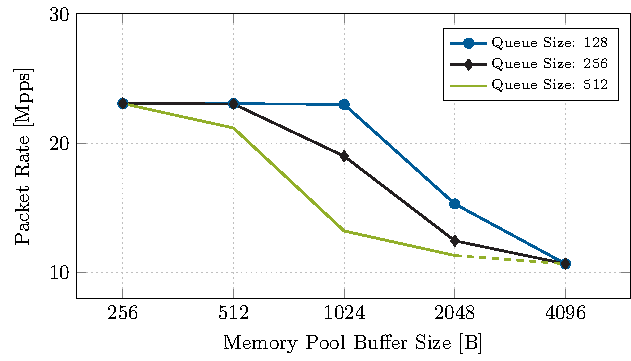
\includegraphics[width=0.46\textwidth]{figures/page-size-4k-omanyte-throughput}

    \caption{Throughput of forwarder on Intel Xeon E5-2620v3 with 4~KiB pages,
    IOMMU enabled, and using a queue for the memory pool.}
	\label{fig:page-size-4k-omanyte}
\end{figure}

As noted before, \Cref{fig:page-size-4k-throughput} and
\Cref{fig:page-size-4k-queue-throughput} depict a drastical loss of performance
with 4~KiB pages and larger memory pool buffer sizes on the Xeon E5 \ac{cpu}
when using the \ac{iommu}. To determine whether this performance degradation is
caused by the number of used pages, we run the forwarder application with
different queue and memory pool buffer sizes on the Xeon E5 \ac{cpu}, using
4~KiB pages, \ac{iommu} and a queue as data structure for the memory pool.
\Cref{fig:page-size-4k-omanyte} shows the results of our measurements.

The stepwise decrease in packet rate for different queue and memory pool buffer
sizes seems to imply that the number of used pages is indeed the reason for loss
of throughput. With 2 + 64~pages per device, i.e., a queue size of 128 and
1,024~B buffers, a queue size of 256 and 512~B buffers or a queue size of 512
and 256~B buffers, throughput is at its maximum. With 2 + 128~pages, packet rate
decreases between 1.9 and 7.7 Mpps. With 2 + 512~pages, throughput is at its
worst with 10.7 Mpps.

\begin{figure}%[!b]
	\centering
	\subfloat[Staggered in time]{%
        \includegraphics[width=0.46\textwidth]{figures/page-size-4k-omanyte-generator-one-throughput}
		\label{fig:page-size-4k-omanyte-generator-one-throughput}
	}
	\subfloat[Concurrently]{%
        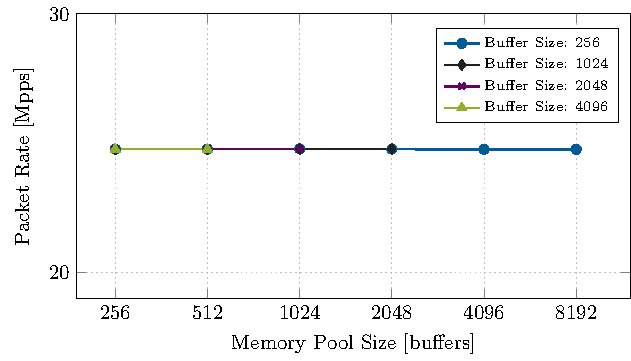
\includegraphics[width=0.46\textwidth]{figures/page-size-4k-omanyte-generator-two-throughput}
		\label{fig:page-size-4k-omanyte-generator-two-throughput}
	}
    \par
	\subfloat[Staggered in time with IOMMU]{%
        \includegraphics[width=0.46\textwidth]{figures/page-size-4k-omanyte-generator-iommu-one-throughput}
		\label{fig:page-size-4k-omanyte-generator-iommu-one-throughput}
	}
	\subfloat[Concurrently with IOMMU]{%
        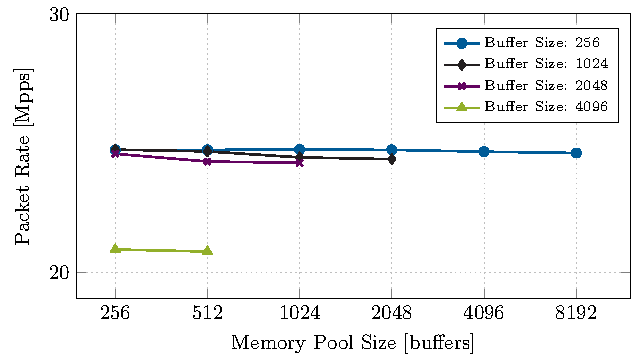
\includegraphics[width=0.46\textwidth]{figures/page-size-4k-omanyte-generator-iommu-two-throughput}
		\label{fig:page-size-4k-omanyte-generator-iommu-two-throughput}
	}

    \caption{Packet rate of two generator instances on Intel Xeon E5-2620v3 with
    4~KiB pages, different memory pool and buffer sizes.}
	\label{fig:page-size-generator}
\end{figure}

We repeat our measurements with the packet generator application on the Xeon E5
\ac{cpu}. \Cref{fig:page-size-generator} shows the results of our measurements.
We use a queue data structure for the memory pool and vary memory pool buffer
and memory pool size to run the generator with different numbers of 4~KiB pages,
ranging from 16~pages (256~buffers with 256~B each) to 512~pages (8,192~buffers
with 256~B each, or 2,048~buffers with 1,024~B each, etc.). We run two instances
of the packet generator, each instance generating traffic on one device. We set
the queue size of RX and TX descriptor ring to 256 entries.
\Cref{fig:page-size-4k-omanyte-generator-one-throughput} and
\Cref{fig:page-size-4k-omanyte-generator-iommu-one-throughput} show the results
when running the generator instances staggered in time,
\Cref{fig:page-size-4k-omanyte-generator-two-throughput} and
\Cref{fig:page-size-4k-omanyte-generator-iommu-two-throughput} when running them
concurrently.

To our surprise, there seems to be no strong correlation between performance
degradation and the number of used pages. Packet rate in the non-\ac{iommu}
measurements is absolutely constant, with a loss of about 40k packets when
running both generators concurrently, while with \ac{iommu}, packet rate
decreases slightly with larger memory pool sizes, and significantly with a
buffer size of 4,096~B. When running the two generators concurrently with
4,096~B buffers, packet rate goes down by 3.7 Mpps compared to 256~B buffers
using the same number of pages.

To verify whether packet rate in \Cref{fig:page-size-4k-omanyte} drops due to
only one \ac{iommu} domain being used for both devices, we modify the forwarder
of \Cref{fig:page-size-4k-omanyte} such that every device belongs to another
domain, and, since the devices can no longer access each other's \ac{dma}
memory, mirror packets received by the devices back onto the link. We check
packet rates in bullet point manner and note that there is almost no difference
in performance (\textasciitilde 0.1~Mpps) when using one or two domains for the
devices. We also modify the packet generator \Cref{fig:page-size-generator} to
generate traffic on two devices, i.e., using only one domain for both devices.
Again, there is no noticeable performance difference between one and two domains
being used.

Our final guess as to why packet rate drops with the forwarder but not the
generator is that while both allocate 512~pages per device, the forwarder uses
both memory pools by each device: packets received by the first device end up in
a memory pool of the first device and are sent out from that pool by the second
device and vice versa. Thus, each device accesses more than 1,024~pages, twice
as many than with the generator. To confirm our suspicion, we modify the
generator such that every device sends out packets in an alternating manner from
two pools. Again, there is no noticeable drop of performance when increasing the
number of pages.

In summary, we note that on the AMD EPYC \ac{cpu}, there are no quantifiable
effects of the \ac{iommu} on performance. On the Intel \acp{cpu}, packet
throughput is impaired by the \ac{iommu} with a performance loss of more than
50\%. However, the reasons for this remain unclear: While our measurements in
\Cref{fig:page-size-4k-omanyte} imply a correlation between packet rate and the
numbers of pages in use, this is not confirmed by our packet generator.


\section{IOVA Address Widths}
\label{sec:iova_address_widths}

For \acp{iova}, any mappings can be chosen. Depending on page size and \ac{iova}
address widths, \acp{iommu} use different paging structures: To translate a
57-bit address to 4~KiB pages, an Intel \ac{iommu} uses a 5-level paging
structure, for 48-bit and 39-bit addresses, 4 and 3 levels are used
respectively.

We run our packet forwarder application to determine the performance impact of
different \ac{iova} address widths. \Cref{fig:iova-address-widths-throughput}
shows the results of our measurements. We run the forwarder on two ports of a
single \ac{nic} (\Cref{fig:iova-address-widths-single-device-throughput}) and on
two distinct \acp{nic} (\Cref{fig:iova-address-widths-two-devices-throughput}).
There are no values for the Intel Xeon E-3 \ac{cpu} and 48-bit addresses as they
exceed the maximum \ac{iova} address widths of the Xeon's \ac{iommu} which is 39
bit.

When using a single dual-ported \ac{nic} for the forwarder, packet rate indeed
decreases by about 1.7 Mpps on both Intel \acp{cpu} with 48-bit addresses
instead of 32-bit addresses. We repeat our measurements and note that the loss
of performance occurs as soon as \ac{iova} address widths surpass the 32-bit
boundary.

When using two \acp{nic} for the forwarder, no significant change in performance
can be observed. Throughput increases slightly on the Intel \acp{cpu} by 0.3
Mpps.

We take a closer look at \Cref{fig:iova-address-widths-single-device-throughput}
with the different packet rates for different \ac{iova} address widths. We note
that 32~bit is not a boundary in the Intel \ac{iommu} paging structure. Compared
to \Cref{fig:iova-address-widths-two-devices-throughput}, throughput of the
forwarder is capped at a certain packet rate. We suspect that this is a
bottleneck at the \ac{pcie} level. A sufficient explanation is given by the
\ac{pcie} specification \cite{pcie2017specification}: The header of \ac{pcie}
memory read requests varies in size depending on the address widths, for 32-bit
addresses it is 4~B smaller. Thus, more packets can be transmitted at the
\ac{pcie} level.

We conclude from these results that changes in performance with different
\ac{iova} address widths are not related to the \acp{iommu}.

\begin{figure}%[!b]
	\centering
	\subfloat[Throughput using 1 NIC]{%
        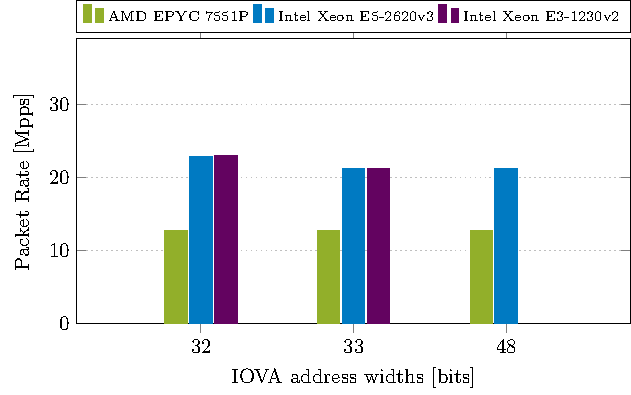
\includegraphics[width=0.46\textwidth]{figures/iova-address-widths-single-device-throughput}
		\label{fig:iova-address-widths-single-device-throughput}
	}
	\subfloat[Throughput using 2 NICs]{%
        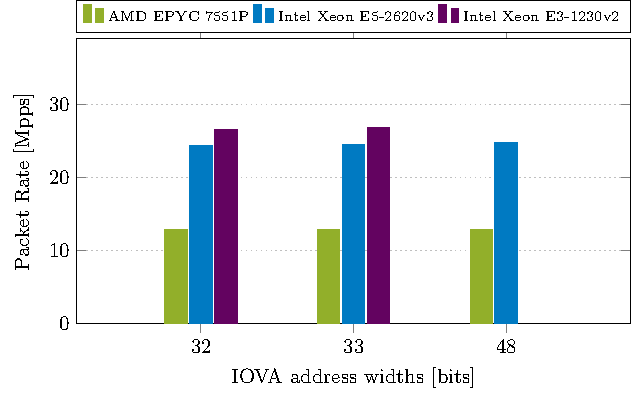
\includegraphics[width=0.46\textwidth]{figures/iova-address-widths-two-devices-throughput}
		\label{fig:iova-address-widths-two-devices-throughput}
	}

    \caption{Throughput of forwarder with 32, 33 and 48 bit wide IOVAs.}
	\label{fig:iova-address-widths-throughput}
\end{figure}


\section{Virtualization}
\label{sec:virtualization}

We take a look at \ac{iommu} impact on virtualization, i.e., \ac{sriov}. For
baseline measurements, we run the packet forwarder and packet generator
application on top of two \acp{vf}, with one \ac{vf} per device. We modify the
applications slightly to work with \ac{sriov}: instead of incrementing one byte
in the packets, the forwarder sets the source \ac{mac} address of each packet to
its own address -- otherwise, packets are dropped by the \ac{nic} due to its
anti-spoofing mechanism.

\Cref{fig:sriov-baseline} shows the results of our measurements. The AMD EPYC
\ac{cpu} is missing as only one of the two \ac{pcie} ports on the board supports
\ac{sriov}. Some values for the Intel Xeon E5 \ac{cpu} are also missing due to
\ac{iommu} group restrictions: On our server, \acp{vf} and \acp{pf} of the
\acp{nic} belong to the same \ac{iommu} group, making it impossible to access
them at the same time by multiple applications through \ac{vfio}, or through
\ac{vfio} and the native driver for the \ac{pf}.

As in our other measurements, two instances of the generator are run for the
measurements, one per device. Notably, compared to the unmodified forwarder in
\Cref{fig:baseline-perf-throughput}, the modified forwarder is about 6~Mpps
slower on the Intel Xeon E5 \ac{cpu}, and about 2~Mpps slower on the Intel Xeon
E3 \ac{cpu}.

The packet rates show that the \acp{iommu} have almost no impact on performance,
neither in the base configuration nor with \acp{vf}. Absurdly, packet rate with
\acp{vf} is 5.3~Mpps greater on the Xeon E5 \ac{cpu} than without \acp{vf}, and
on the Xeon E3 \ac{cpu} the forwarder with \acp{vf} reaches a new maximum of all
measurements with 27.6~Mpps (0.15~Mpps faster compared to
\Cref{fig:baseline-perf}).

\begin{figure}%[!b]
	\centering
	\subfloat[Throughput on Intel Xeon E5-2620v3]{%
        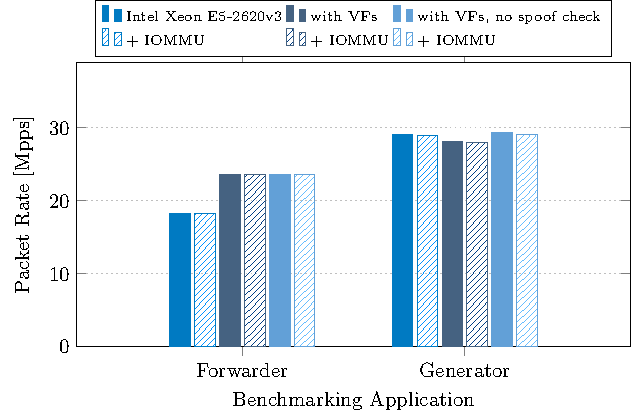
\includegraphics[width=0.49\textwidth]{figures/sriov-omanyte-throughput}
		\label{fig:sriov-omanyte-throughput}
	}
    \subfloat[Throughput on Intel Xeon E3-1230v2]{%
        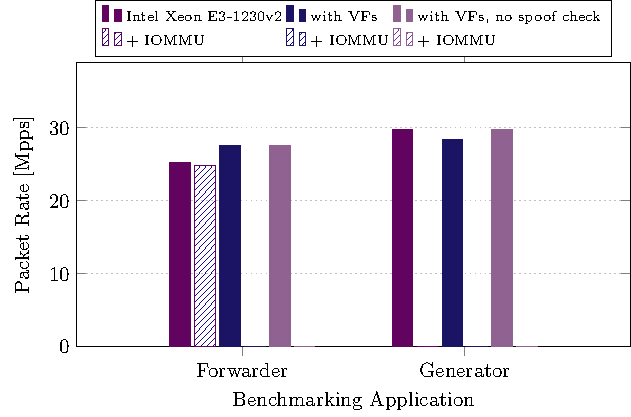
\includegraphics[width=0.49\textwidth]{figures/sriov-narva-throughput}
		\label{fig:sriov-narva-throughput}
	}
    \par
	\subfloat[Latency on Intel Xeon E5-2620v3]{%
        \includegraphics[width=0.49\textwidth]{figures/sriov-omanyte-latency}
		\label{fig:sriov-omanyte-latency}
	}
	\subfloat[Latency on Intel Xeon E3-1230v2]{%
        \includegraphics[width=0.49\textwidth]{figures/sriov-narva-latency}
		\label{fig:sriov-narva-latency}
	}

    \caption{Throughput and latency of modified forwarder with two devices, with
    and without VFs, with and without IOMMU. Latency of forwarder measured with
    a total packet rate of 10 Mpps.}
	\label{fig:sriov-baseline}
\end{figure}

When running the generator application, we note that throughput is capped at
14.20~Mpps per port. We disable the \ac{mac} anti-spoofing mechanism and reach
line rate on the Xeon E3 \ac{cpu}, i.e., 14.88~Mpps per port. Thus, we put the
cost of the spoof check at 0.68 Mpps per port or 1.36 Mpps in total. We repeat
this experiment on the AMD EPYC \ac{cpu} and note that packet rate increases
from 14.08~Mpps to 14.35~Mpps when disabling the spoof check. To our surprise,
on all hosts the \ac{pf} driver of the Linux kernel reports some spoofed packets
when switching the spoof check on or off on the fly.

We also measure the latency. On the Xeon E3, latency of forwarder, and forwarder
with \acp{vf} resemble each other with, while latency of forwarder with
\ac{iommu} is on average 1 microsecond greater than without \ac{iommu}. On the
Xeon E5, latencies are also approximately the same, but tail latencies diverge.
Interestingly, forwarder and \ac{iommu} achieve the lowest tail latencies,
followed by the forwarder as-is, forwarder with \acp{vf} and forwarder with
\acp{vf} and \ac{iommu}.

We conclude that \acp{iommu} do not have a significant effect on throughput and
latency of \acp{vf}.


\section{Summary}
\label{sec:perf_summary}

Regarding the AMD EPYC \ac{cpu}, there are no measurable differences in
performance with AMD's \ac{iommu}. On Intel systems, \acp{iommu} have a negative
impact on performance in certain configurations. We suspect a correlation
between throughput and the amount of pages used by a device. To be more precise,
we assume that the \ac{iotlb} gets thrashed the more pages are used.

This assumption is not unreasonable: The datasheet for the Intel 82599 \acp{nic}
mentions changes in the \ac{pcie} transaction size to decrease the number of
\ac{pcie} transactions and thus thrashing of the \ac{iotlb}
\cite[p.~34]{intel2019datasheet}. And Neugebauer et al.
\cite{neugebauer2018understanding} report \ac{iotlb} thrashing on their Intel
Xeon E5-2630v4 based system, and determine an \ac{iotlb} size of 64 entries for
that particular \ac{iommu}. Unfortunately, our measurements confirm the
correlation between throughput and used pages only to some extent.

We were not able to identify any striking performance differences in relation to
\ac{iova} addresses or virtualization.



\chapter{Safety and Security}
\label{chap:safety_and_security}

\acp{iommu} have been bypassed in numerous ways due to weaknesses in \ac{pcie},
boot-time issues and poor configuration of \acp{iommu} by \acp{os}. We will
describe some attacks to give a short overview of vulnerabilities. In the second
half of the chapter (\Cref{sec:iotlb}), we will take a closer look at the
\ac{iotlb} of \acp{iommu} which we assume to be another weak point. We suspect
that the \ac{iotlb} is susceptible to timing attacks.


\section{Known Vulnerabilities}
\label{sec:known_vulnerabilities}

On the \ac{pcie} level, two flaws stand out. First, devices can impersonate
other \ac{pcie} devices by spoofing their \ac{pcie} ID (i.e., the \ac{bdf}).
Since \acp{iommu} perform address translation and check access permissions based
on the \ac{pcie} ID of \ac{pcie} packets, devices can access memory assigned to
other devices by spoofing their ID. When \acp{iommu} are used in pass-through
mode, i.e., only some devices use the \ac{iommu}, devices may even bypass the
\ac{iommu} completely and access all memory of a host. Access in this context
refers primarily to write access. For read access, routing configuration has to
be updated. This is theoretically possible but rather unlikely in practice.
Daubignard and Perez explain the attack vector in more detail
\cite{daubignard2017protip}.

Second, devices may implement a \ac{pcie} capability called Address Translation
Services (ATS). With ATS, devices announce that they are capable of caching
address translations and translate addresses of \ac{dma} requests on their own.
Thus, ATS reduces pressure on the \ac{iotlb} of \acp{iommu}. Devices using this
capability request translations from \ac{dma} remapping hardware, cache the
translations and receive invalidation requests once address mappings are no
longer valid. \ac{pcie} memory read and write requests of such devices indicate
whether the specified address was translated by the device or still needs to be
translated (by the \ac{iommu}). If ATS is enabled for a device, memory requests
with translated addresses pass the remapping hardware unchecked. There are no
restrictions on which addresses can be accessed by a device, malicious or faulty
devices can masquerade any address as legitimately translated address.

Both flaws in the \ac{pcie} protocol can be mitigated (to a certain point) using
a \ac{pcie} feature named Access Control Services (ACS). With ACS, ports of the
root complex and switches can be configured to verify whether the \ac{pcie} ID
used in a request belongs to a port's subset of bus numbers. Furthermore, memory
requests with ATS-translated addresses can be blocked. These operations are
known as source validation and translation blocking. However, ACS is an optional
\ac{pcie} feature and might not or only partially be available on a system
\cite[p.~582]{pcie2017specification}.

In case ACS is not available, ATS can still be disabled in the \ac{iommu}. Both
Intel's and AMD's \acp{iommu} check memory requests with translated addresses
for eligibility, i.e., whether ATS is enabled. Intel stores this information in
the context entry of the domain, AMD in the device entry.

Other attack vectors exist at boot-time: On some architectures, \acp{iommu}
could be hidden from the \ac{os} by rewriting the \ac{dmar} \ac{acpi} tables at
boot-time \cite{wojtczuk2009another}. Morgen et al. used another weakness and
rewrote the tables of the \ac{iommu} during initialization, setting the
translation type of \ac{iommu} domains to pass-through mode
\cite{morgan2018iommu}.

The flaws in how \aclp{os} configure \acp{iommu} are even worse. In 2019,
Markettos et al. examined the behavior of all major \acp{os} and came to
disillusioning conclusions \cite{markettos2019thunderclap}. Most versions of
Microsoft Windows did not use the \ac{iommu} at all and were therefore entirely
unprotected against \ac{dma} attacks. Windows 10 Enterprise supported
\acp{iommu}, however, they were only used to protect a secure container (VBS),
not the root operating system. Unlike Windows, macOS and Linux enabled
\acp{iommu}. However, \ac{dma} memory was shared between devices on macOS and
both \aclp{os} exposed \ac{os} data structures to the devices. Markettos et al.
show 5 different ways on macOS and Linux to bypass the \ac{iommu}, some so
serious that a root shell could be obtained.

Following the revelations of Markettos et al., \ac{os} vendors released
mitigations against the newly discovered vulnerabilities. Besides, Microsoft
announced to support \acp{iommu} as of Windows 10 version 1803, and Linux
disabled ATS entirely for external devices (e.g., Thunderbolt). However,
internal hardware is still considered trustworthy. To reduce the surface area
for attacks sustainably, Markettos et al. call for a fundamental change of the
thread models of operating systems and drivers.


\section{The IOTLB}
\label{sec:iotlb}

We suspect that there exists yet another vulnerability in \acp{iommu} in
relation to \acp{iotlb}, which are used by \acp{iommu} to cache information
about domains and address mappings to accelerate address lookup. To be more
precise, we suspect that these \acp{iotlb} -- just like other caches -- are
vulnerable to timing attacks, i.e., multiple devices or functions share the same
\ac{iotlb} and \ac{dma} access times depend on availability of translation
information in the cache.

We implement an application on top of the methods described in
\Cref{sec:iommu_leaks} to run some timing measurements on \ac{dma} operations.
Our application follows the idea of priming and probing: By carefully
controlling the \ac{dma} accesses of the \ac{nic}, we try to bring the
\ac{iotlb} into a known state. We run our measurements on the Intel Xeon E5
\ac{cpu} as it is the only \ac{cpu} that supports \ac{sriov} with \ac{iommu} and
two devices.

We assume that the \ac{iotlb} of this \ac{cpu} has 64 entries. We allocate 64
physically and virtually contiguous 4~KiB pages, place the TX descriptor ring on
the first page and use the other 63 pages for our packets. We use one port of
the Intel X520-DA2 \ac{nic} for our application and configure the device to use
our 64 pages. We disable the RX queue of the device to prevent \ac{dma} accesses
on packet arrival.

\begin{figure}%[!b]
    \centering
    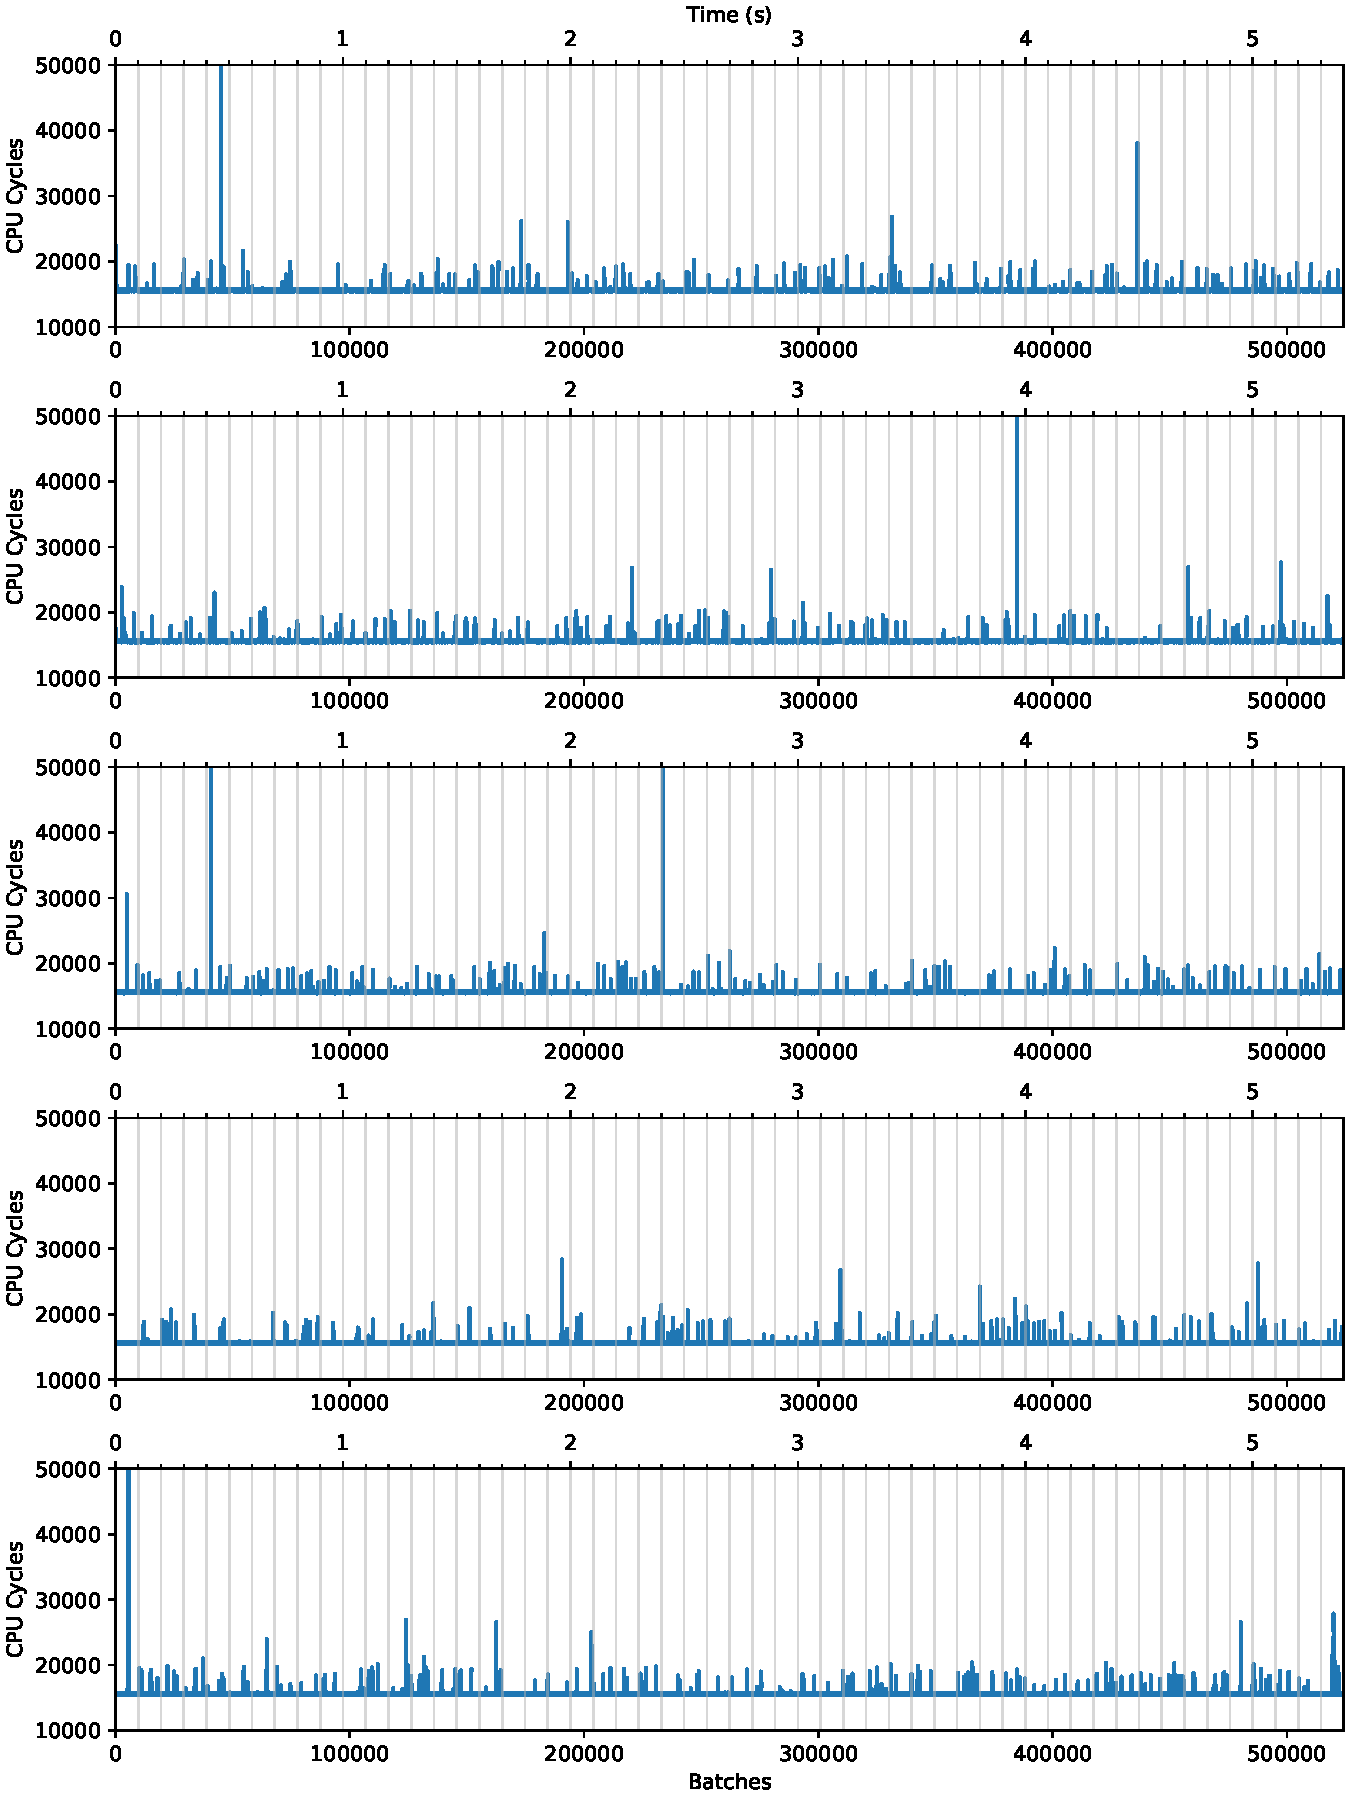
\includegraphics[width=1.0\textwidth]{figures/iotlb-baseline-no-iommu}
    \caption{CPU cycles per batch of transmitted packets.}
    \label{fig:cycles-no-iommu}
\end{figure}

\begin{figure}%[!b]
    \centering
    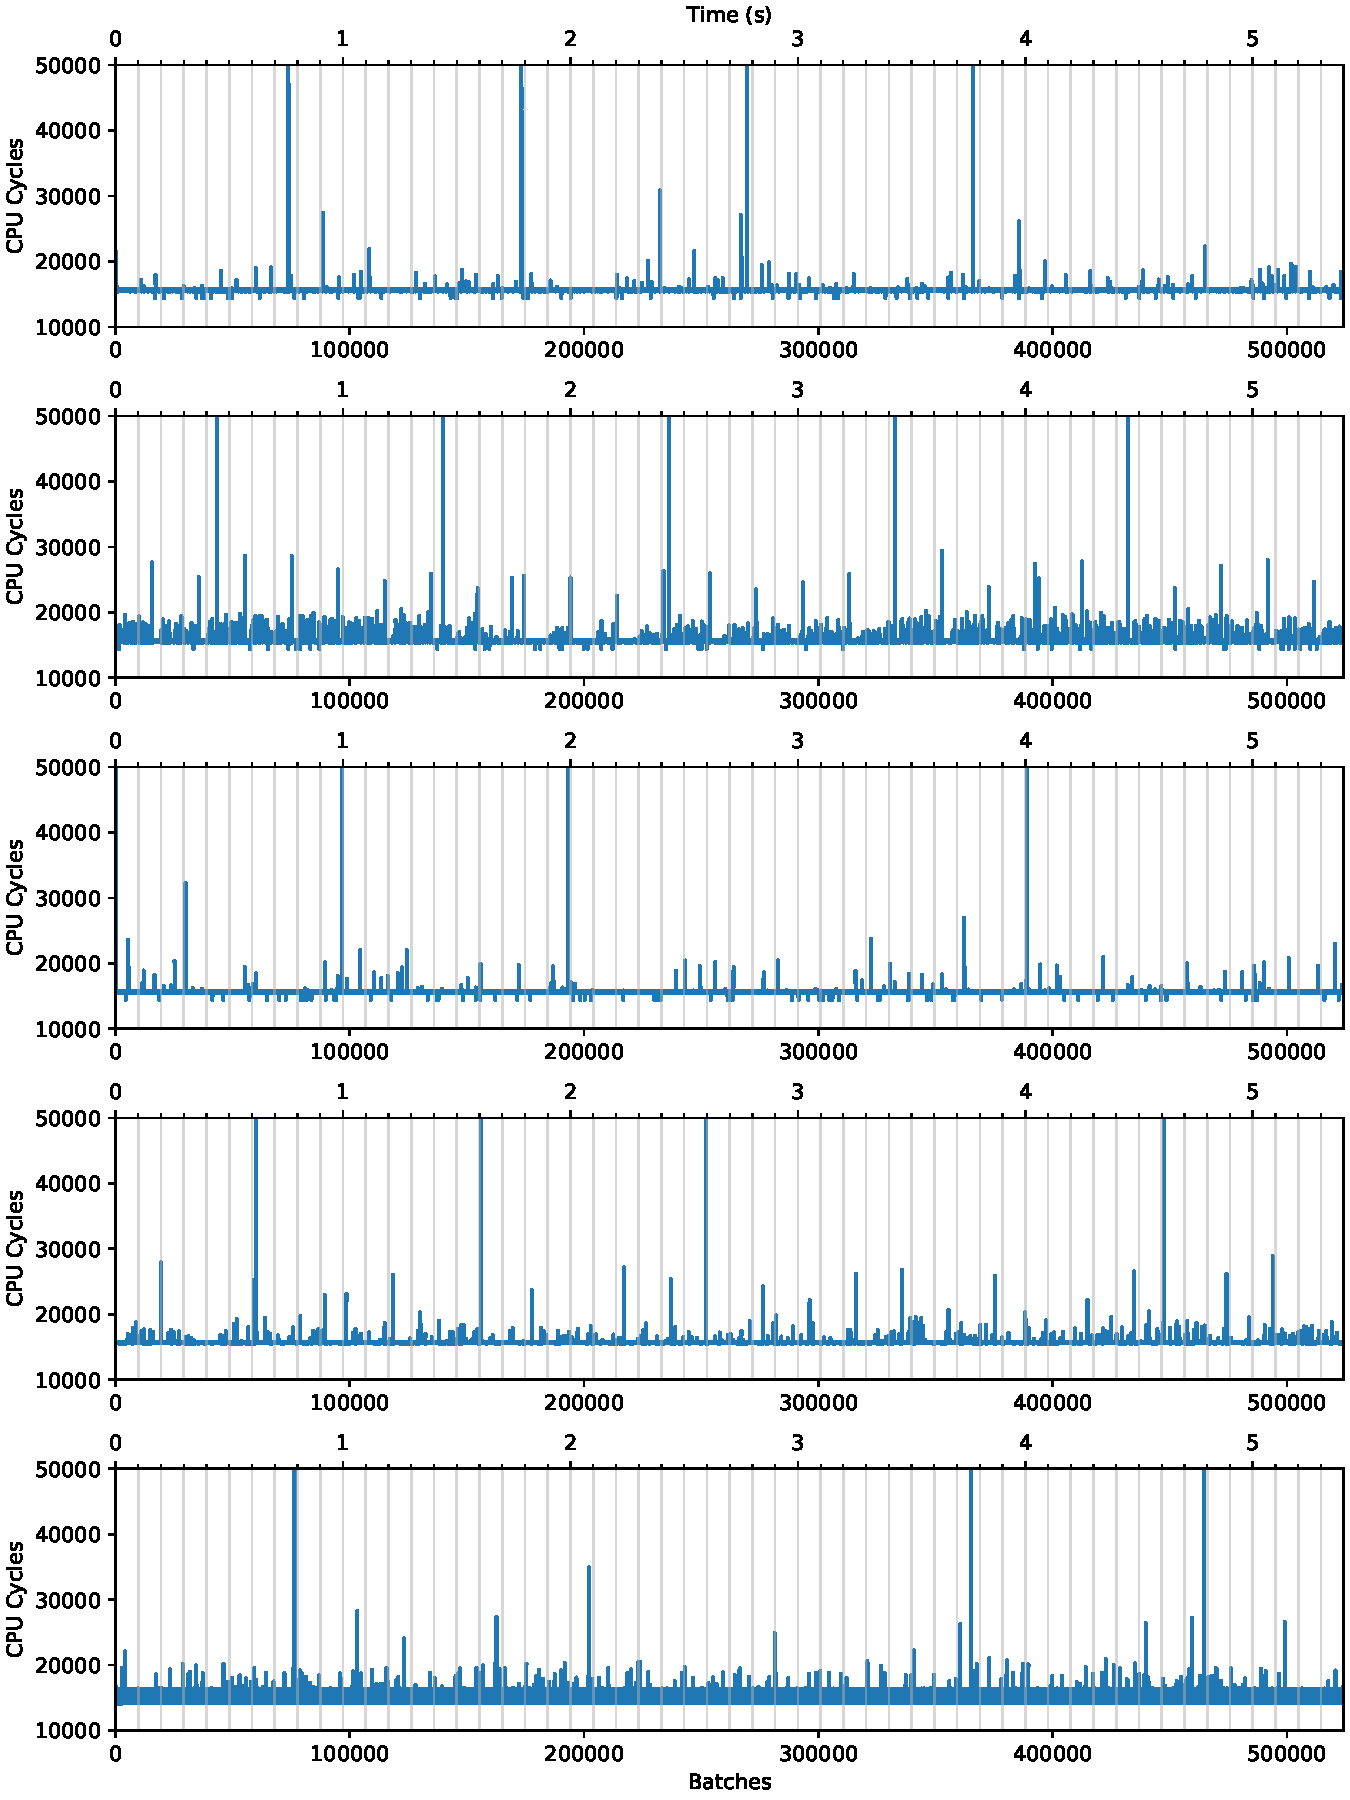
\includegraphics[width=1.0\textwidth]{figures/iotlb-baseline-iommu-pt}
    \caption{CPU cycles per batch of transmitted packets with IOMMU.}
    \label{fig:cycles-iommu-pt}
\end{figure}

\begin{figure}%[!b]
    \centering
    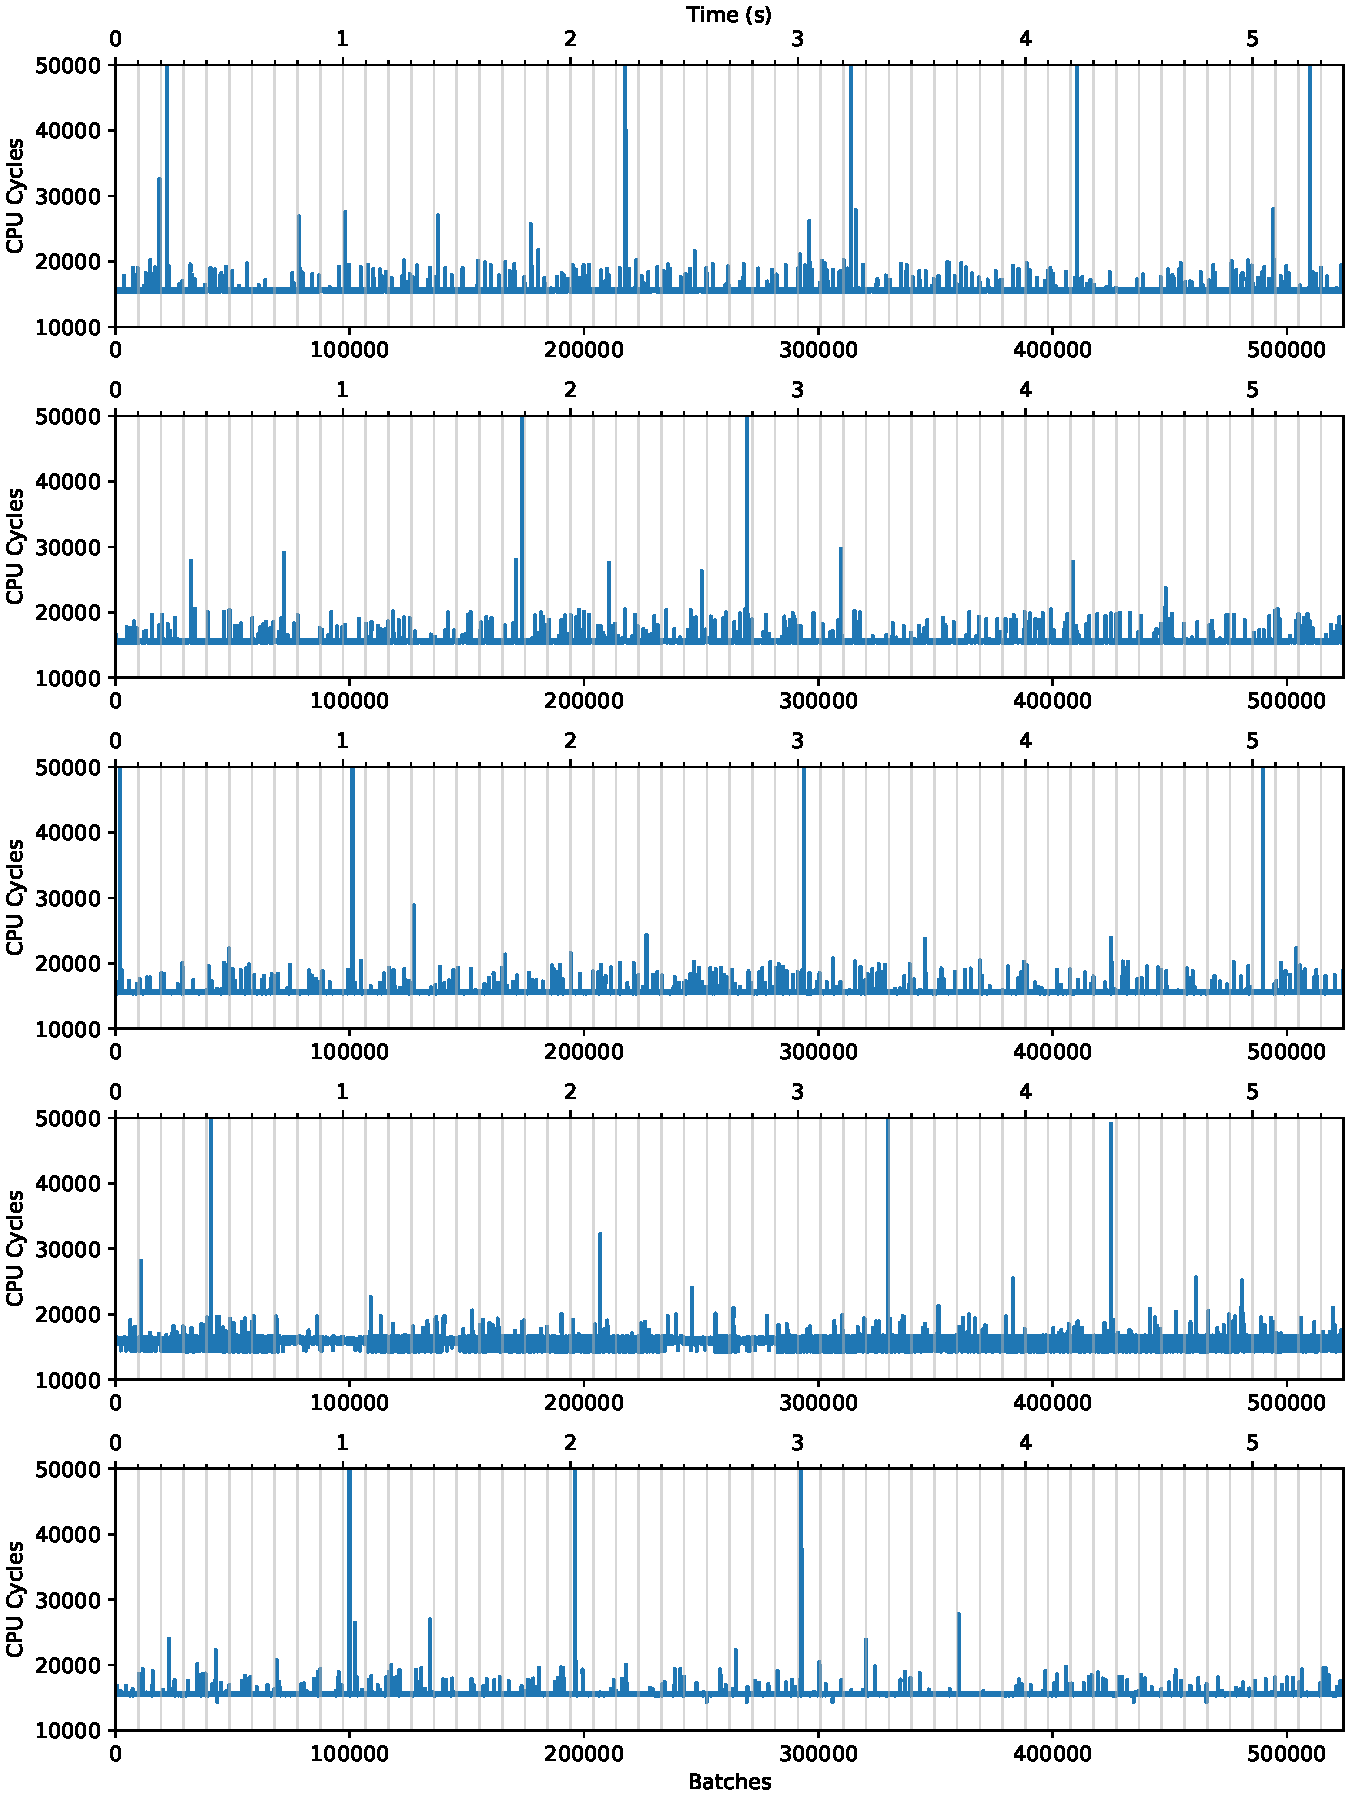
\includegraphics[width=1.0\textwidth]{figures/iotlb-baseline-iommu-pt-fixed}
    \caption{CPU cycles per batch of transmitted packets with IOMMU and fixed
virtual and physical addresses.}
    \label{fig:cycles-iommu-pt-fixed}
\end{figure}

In our first measurements, we try to determine the number of \ac{cpu} cycles it
takes for the \ac{nic} to fetch the TX descriptors from one page, transmit a
batch of 63 packets from the 63 other pages, and set the descriptor-done bit in
the last TX descriptor on the descriptor page. Thus, the \ac{nic} accesses 64
distinct but physically and virtually contiguous pages for every batch of
to-be-transmitted packets.

We run the application with and without \ac{iommu}. We warm up the caches before
starting our measurements. For every run of the application, we measure the
\ac{cpu} cycles for 500k batches and mean and standard deviation of the
\ac{cpu} cycles. \Cref{fig:cycles-no-iommu} shows the results of five runs
without \ac{iommu}. The plots are cut off at 50,000~\ac{cpu} cycles, all spikes
that end up at 50,000 cycles go up to 400,000 \ac{cpu} cycles.

Several conclusions can be drawn from the plots. First, the number of \ac{cpu}
cycles varies greatly in every run. Second, the number of \ac{cpu} cycles
between spikes is constant in a run and for all runs. Third, some spikes appear
equidistantly across runs, e.g., with a time interval of 0.4, 0.6 or 2.0s.

On average, we note 15,622 \ac{cpu} cycles and a standard deviation of
623~cycles for the runs in \Cref{fig:cycles-no-iommu}. With a batch size of
63~packets, we get 248~cycles per packet.

We repeat our measurements with the \ac{iommu} in pass-through mode, i.e., only
our device uses the \ac{iommu}. \Cref{fig:cycles-iommu-pt} shows the results.
Notably, variance of the \ac{cpu} cycles is even worse with \ac{iommu}. However,
we can also notice more patterns in the spikes. In the second run from the top,
spikes between 22k and 30k \ac{cpu} cycles appear every 0.2 seconds, and spikes
above 50,000 \ac{cpu} cycles every second.

On average, we note 15,682 \ac{cpu} cycles and a standard deviation of
658~cycles for the runs in \Cref{fig:cycles-iommu-pt}. With a batch size of
63~packets, we get 249~cycles per packet. Thus, we put the cost of the
\ac{iommu} at 60~cycles per batch of packets or about 1~cycle per packet.

To minimize variance between runs, we modify our application such that the same
virtual and physical memory addresses are used for every run. We allocate a
chunk of physical memory on boot using the Linux kernel's \texttt{memmap} flag
and \texttt{mmap} the memory chunk into the process address space via
\texttt{/dev/mem}.

\Cref{fig:cycles-iommu-pt-fixed} shows the results of running our application
with \ac{iommu} and fixed addresses. To our disappointment, \ac{cpu} cycles
still vary greatly although all runs were executed on the same \ac{cpu} core
with the same memory addresses and no dynamic overclocking. Again, we note a
periodicity of the peaks of 1.0 and 2.0 seconds.


\section{Summary}
\label{sec:sec_summary}

\acp{iommu} provide limited protection against malicious or faulty peripherals
due to weaknesses in the \ac{pcie} protocol. Besides, architectural flaws,
missing support and incorrect handling of \acp{iommu} by \aclp{os} further
reduce the safety / security benefits of employing \acp{iommu}.

Although we suspect the possiblity of side-channel attacks using the \ac{iotlb},
our timing measurements in \Cref{sec:iotlb} do not reveal any significant
differences between non-\ac{iommu} and \ac{iommu} usage. Our measurements prove
to have far too much variance to detect any individual \ac{iotlb} misses.



\chapter{Conclusion}
\label{chap:conclusion}

We investigated the effects of hardware isolation in high-speed network
environments with a focus on Intel's and AMD's \acp{iommu}. We used the
\texttt{ixy.rs} user space network driver for our analyses, and adapted it to
our needs. We implemented support for multiple devices in an \ac{iommu} group
and \acp{iommu} with limited IOVA translation capabilities. We also implemented
a whole new driver in \texttt{ixy.rs} for virtual functions, \texttt{ixgbevf}.
And we implemented methods for precise timing measurements on \ac{nic}
operations to investigate the \ac{iotlb} of \acp{iommu}, including a brute-force
memory allocator to allocate physically contiguous memory in user space.

Our findings with \texttt{ixy.rs} paint a multi-layered picture of \acp{iommu}.
In regards to performance, our results show that on most configurations, neither
throughput nor latency are affected by \acp{iommu} to a quantifiable extent, be
it in virtualized or non-virtualized environments. There are, however, some
configurations where \acp{iommu} have a negative impact, leading to a loss of
packet throughput of more than 50\%.

In regards to safety and security, our picture of \acp{iommu} is rather bleak:
Against common believe, \acp{iommu} do not protect against malicious or faulty
peripherals due to the weaknesses in the \ac{pcie} protocol and archaic threat
models of \ac{os} vendors which see internal \ac{io} peripherals as trustworthy
and enable inherently unsafe features like ATS on these devices.

As a result, many weaknesses in the handling of \acp{iommu} have been uncovered
in the past, as well as some architectural deficiencies. We believe that more
vulnerabilities are to be discovered and suspect one in the hardware of
\acp{iommu}: the \ac{iotlb}. As other caches, we believe that the \ac{iotlb} is
susceptible to timing attacks and thus provides an attack surface for side
channel attacks. If timing of \ac{dma} accesses and address translation through
the \ac{iotlb} can be measured precisely, packet receival and transmittal times
of other devices sharing the \ac{iotlb} could be leaked.

Our measurements on \ac{dma} operations provide some insight on the performance
characteristics of Intel's \ac{iommu}. We hope these results can be used in the
future to uncover the suspected vulnerability in the \ac{iotlb}.

Generally speaking of safety and security, however, we recognize that a lot has
changed in the last years: More and more \acp{os} support \acp{iommu} or improve
their usage of \acp{iommu} when mitigating vulnerabilities, more vendors of
consumer products include \acp{iommu} into their hardware to protect systems
against external peripherals, and even on mobile phones \acp{iommu} are on the
rise: Apple has developed its own \ac{iommu} for the iPhone, Google uses an
\ac{iommu} on the Pixel phones, and ARM-based Android phones often have an ARM
SMMU included.

In view of these rapid changes, we believe that effects of hardware isolation
remain an exciting research topic in all kinds of environments, not necessarily
restricted to virtualization and high-speed networking.


\section{Future Work}
\label{chap:future_work}

Future work could continue our work on the \ac{iotlb}, investigate \acp{iommu}
on mobile platforms, e.g., the \ac{iommu} of Apple's iPhones, or focus on
Linux's VFIO API and its different ways of handling IOVA address mappings, e.g.,
coalescing of addresses and mapping with different page sizes.




\appendix

\listoffigures
\listoftables
\lstlistoflistings

\printacronyms[heading=chapter,name=List of acronyms]
\clearpage
\pagestyle{thesischapter}

\cleardoublepage
\printbibliography[heading=bibintoc]

\clearpage
\pagestyle{empty}

\end{document}


